
\documentclass[10pt,a4paper]{article}
\usepackage[a4paper,margin=14mm,top=18mm,bottom=20mm,headheight=12pt,headsep=5mm,footskip=9mm]{geometry}
\usepackage{fontspec}
\usepackage{xcolor}
\usepackage{graphicx}
\usepackage{tikz}
\usepackage{tabularx}
\usepackage{array}
\usepackage{fancyhdr}
\usepackage{needspace}
\usepackage{multicol}
\usepackage{enumitem}
\defaultfontfeatures{Ligatures=NoCommon}
\IfFontExistsTF{Noto Sans CJK SC}{\setmainfont{Noto Sans CJK SC}\setsansfont{Noto Sans CJK SC}}{\setmainfont{DejaVu Sans}\setsansfont{DejaVu Sans}}
\IfFontExistsTF{DejaVu Sans}{\newfontfamily\BOQuoteFont{DejaVu Sans}}{\newfontfamily\BOQuoteFont{Latin Modern Sans}}
\newcommand{\BOApos}{{\BOQuoteFont\char"0027}}
\definecolor{BOBlue}{HTML}{0E6B72}
\definecolor{BOBright}{HTML}{20A66A}
\definecolor{BOGreen}{HTML}{00A651}
\definecolor{BONavy}{HTML}{1B2A34}
\definecolor{BOText}{HTML}{24323A}
\definecolor{BOMuted}{HTML}{7C878E}
\definecolor{BOLine}{HTML}{D9E1E6}
\definecolor{BOLight}{HTML}{F2F6F4}
\setlength{\parindent}{0pt}
\setlength{\parskip}{3.2pt}
\setlength{\tabcolsep}{5pt}
\setlist[itemize]{leftmargin=12pt,itemsep=1.5pt,topsep=2pt,parsep=0pt}
\renewcommand{\arraystretch}{1.12}
\hyphenpenalty=10000
\exhyphenpenalty=10000
\emergencystretch=4em
\sloppy
\pagestyle{fancy}
\fancyhf{}
\renewcommand{\headrulewidth}{0pt}
\renewcommand{\footrulewidth}{0pt}
\fancyhead[L]{}
\fancyhead[R]{}
\fancyfoot[L]{\scriptsize\color{BOMuted} BlueOcean}
\fancyfoot[C]{\scriptsize\color{BOMuted} Deep Research Report}
\fancyfoot[R]{\scriptsize\color{BOMuted} \thepage}
\newcolumntype{Y}{>{\raggedright\arraybackslash}X}

\begin{document}
\raggedright

\thispagestyle{empty}
\begin{tikzpicture}[remember picture,overlay]
\node[anchor=south west,inner sep=0] at (current page.south west) {
\includegraphics[width=\paperwidth,height=\paperheight]{assets/cover-ai.png}};
\fill[BONavy,opacity=.10] (current page.south west) rectangle (current page.north east);
\fill[white,opacity=.96] ([xshift=14mm,yshift=-24mm]current page.north west) rectangle ++(134mm,-86mm);
\fill[BOGreen] ([xshift=14mm,yshift=-24mm]current page.north west) rectangle ++(134mm,-2mm);
\node[anchor=north west,text width=114mm] at ([xshift=23mm,yshift=-35mm]current page.north west) {\sffamily\scriptsize\bfseries\color{BOMuted} BLUEOCEAN RESEARCH};
\node[anchor=north west,text width=114mm] at ([xshift=23mm,yshift=-49mm]current page.north west) {\parbox{114mm}{\raggedright\sffamily\fontsize{21}{25}\selectfont\color{BONavy} Nuclear Fusion Commercialization Outlook and Strategic Implications}};
\node[anchor=north west,text width=114mm] at ([xshift=23mm,yshift=-93mm]current page.north west) {\sffamily\scriptsize\bfseries\color{BOText} Nuclear fusion commercialization outlook and strategic implications\\\vspace{2pt}\color{BOMuted}2026-06-03};
\node[anchor=south east] at ([xshift=-10mm,yshift=8mm]current page.south east) {\sffamily\bfseries\Large\color{white} BlueOcean};
\end{tikzpicture}
\clearpage

\clearpage
{\sffamily\fontsize{26}{31}\selectfont\color{BONavy} Contents}\par\vspace{10pt}
\begin{tabularx}{\linewidth}{p{14mm}Y}
\textcolor{BOGreen}{\bfseries 03} & Nuclear fusion is approaching technical viability \\[5pt]
\textcolor{BOGreen}{\bfseries 04} & The case should be read through proof, economics and timing \\[5pt]
\textcolor{BOGreen}{\bfseries 05} & The first evidence pages frame decision readiness before the narrative \\[5pt]
\textcolor{BOGreen}{\bfseries 07} & Nuclear Fusion Is Approaching Technical Viability but Commercial Deployment Remains Over a Decade Away \\[5pt]
\textcolor{BOGreen}{\bfseries 09} & Magnetic Confinement Leads in Maturity but Faces High Capital Costs and Long Construction Times \\[5pt]
\textcolor{BOGreen}{\bfseries 11} & Private Fusion Companies Are Accelerating Timelines with Innovative Designs and Substantial Funding \\[5pt]
\textcolor{BOGreen}{\bfseries 12} & Regulatory and Licensing Frameworks Are Underdeveloped, Posing Significant Timeline Risks \\[5pt]
\textcolor{BOGreen}{\bfseries 14} & Fusion\BOApos{}s Strategic Value Lies in Baseload Clean Power and Energy Independence, Not Near-Term Disruption \\[5pt]
\textcolor{BOGreen}{\bfseries 15} & Falling Costs of Renewables and Storage May Erode Fusion\BOApos{}s Competitive Advantage \\[5pt]
\textcolor{BOGreen}{\bfseries 17} & Geopolitical Dynamics Are Shaping Fusion R\&D Leadership \\[5pt]
\textcolor{BOGreen}{\bfseries 18} & Recommendations for Decision-Makers \\[5pt]
\textcolor{BOGreen}{\bfseries 20} & About the research \\[5pt]
\end{tabularx}
\clearpage

\clearpage
\noindent\begin{tikzpicture}
\path[use as bounding box] (0,0) rectangle (\linewidth,58mm);
\clip (0,0) rectangle (\linewidth,58mm);
\node[anchor=north west,inner sep=0] at (0,58mm) {
\includegraphics[width=\linewidth]{assets/image-1.png}};
\end{tikzpicture}
\vspace{0pt}
\noindent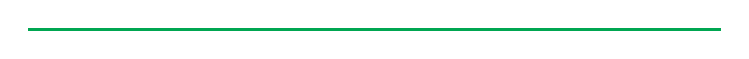
\begin{tikzpicture}
\fill[BOGreen] (0,0) rectangle (88mm,1.2pt);
\end{tikzpicture}\par\vspace{8pt}
{\sffamily\fontsize{24}{30}\selectfont\color{BONavy} Nuclear fusion is approaching technical viability}\par\vspace{11pt}
\begin{minipage}[t]{0.44\linewidth}
{\sffamily\fontsize{17}{23}\selectfont\color{BOGreen} Nuclear fusion is approaching technical viability}\par\vspace{10pt}
{\small\color{BOText} Nuclear fusion is approaching technical viability, but commercial deployment remains over a decade away. The decision to invest or develop a strategic position hinges on understanding which fusion approaches are most promising, the realistic timelines, and the regulatory and market risks. This report synthesizes public-source evidence to conclude that while fusion will not disrupt energy markets before 2040, its strategic value as a baseload clean power source and enabler of energy independence justifies selective investment now. The immediate next step is to build a diversified portfolio of leading private ventures and enabling technologies, while closely monitoring milestones from ITER, SPARC, and other key projects. Regulatory and licensing frameworks are underdeveloped and pose significant timeline risks; early engagement with regulators is critical. Falling costs of renewables and storage may erode fusion\BOApos{}s competitive advantage if fusion costs do not decline as projected; benchmark fusion cost targets against realistic future energy prices.}\par
\end{minipage}\hfill\begin{minipage}[t]{0.45\linewidth}
{\small\color{BOText} This report synthesizes public-source evidence to conclude that while fusion will not disrupt energy markets before 2040, its strategic value as a baseload clean power source and enabler of energy independence justifies selective investment now. The immediate next step is to build a diversified portfolio of leading private ventures and enabling technologies, while closely monitoring milestones from ITER, SPARC, and other key projects. Regulatory and licensing frameworks are underdeveloped and pose significant timeline risks; early engagement with regulators is critical.}\par
\end{minipage}

\clearpage
\noindent\begin{tikzpicture}
\path[use as bounding box] (0,0) rectangle (\linewidth,62mm);
\clip (0,0) rectangle (\linewidth,62mm);
\node[anchor=north west,inner sep=0] at (0,62mm) {
\includegraphics[width=\linewidth]{assets/image-2.png}};
\end{tikzpicture}
\vspace{0pt}
\noindent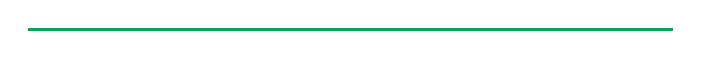
\begin{tikzpicture}
\fill[BOGreen] (0,0) rectangle (82mm,1.2pt);
\end{tikzpicture}\par\vspace{8pt}
{\sffamily\fontsize{23}{29}\selectfont\color{BONavy} Nuclear Fusion Is Approaching Technical Viability but Commercial Deployment Remains Over a Decade Away}\par\vspace{8pt}
{\sffamily\fontsize{16}{21}\selectfont\color{BOGreen} Fusion\BOApos{}s scientific feasibility has been proven, but the path to commercial power plants is long and uncertain, requiring patient capital and milestone-based investment.}\par\vspace{9pt}
\begin{minipage}[t]{0.46\linewidth}
{\small Magnetic confinement fusion, particularly tokamaks, is the most mature approach but faces high capital costs and long construction times. ITER, the largest tokamak experiment, has been under construction since 2013 and is not expected to achieve full fusion power until the 2030s. Private ventures like Commonwealth Fusion Systems aim to accelerate timelines with high-temperature superconducting magnets. Investments in magnetic confinement should be patient and milestone-based, with clear exit options if delays}\par
{\small Regulatory and licensing frameworks for fusion are underdeveloped, posing significant timeline risks. The U.S. Nuclear Regulatory Commission has not yet established a licensing framework for fusion reactors. The National Academies study \BOApos{}Bringing Fusion to the U.S. Grid\BOApos{} highlights this as a critical gap. Engage early with regulators and support the development of clear, fusion-specific rules to avoid delays.}\par
\end{minipage}\hfill\begin{minipage}[t]{0.46\linewidth}
{\small Private fusion companies are attracting significant funding and claim accelerated timelines, but their claims remain unverified at scale. Fusion Industry Association reports indicate over \$6 billion in private fusion investment since 2015. Companies like Helion Energy and TAE Technologies target commercial reactors by the early 2030s, but no private company has yet demonstrated net energy gain in a reactor-relevant configuration. Due diligence must focus on technical milestones, not just funding amounts}\par
{\small Fusion\BOApos{}s strategic value lies in baseload clean power and energy independence, not near-term disruption. Fusion offers continuous power with no carbon emissions and minimal waste, complementing intermittent renewables. It could reduce dependence on fossil fuel imports and enhance national security. Position fusion as a long-term hedge in energy portfolios, not a near-term competitor to solar or wind.}\par
\end{minipage}

\clearpage
{\textcolor{BOGreen}{\scriptsize\bfseries EXHIBIT 1}}\par\vspace{4pt}
{\sffamily\fontsize{17}{21}\selectfont\color{BONavy} Decision readiness still depends on verified proof points}\par
{\small\color{BOText} Customer, cost and partner proof remain the main underwriting gaps for Nuclear Fusion Commercialization Outlook and Strategic Implications}\par\vspace{6pt}
\noindent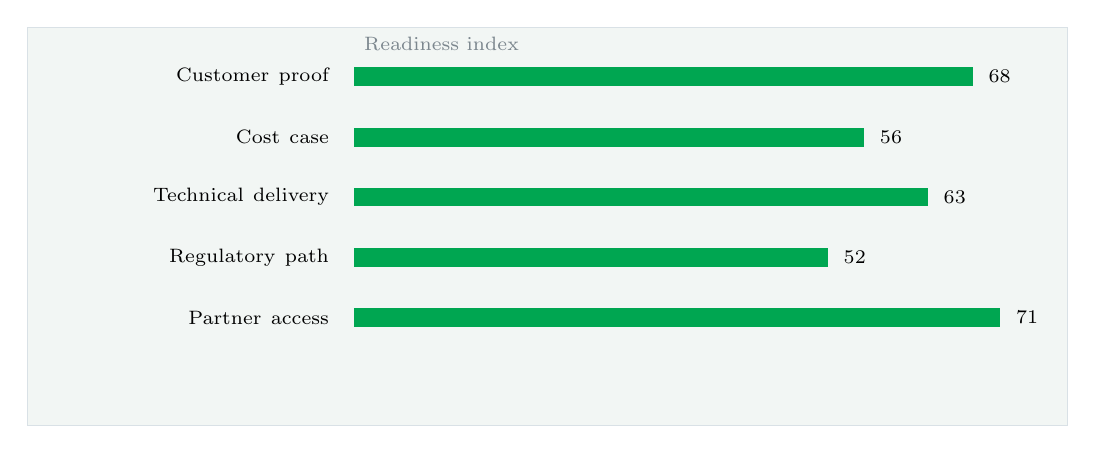
\begin{tikzpicture}[x=1cm,y=1cm]
\path[use as bounding box] (0,0) rectangle (13.20,5.05);
\fill[BOLight] (0,0) rectangle (13.20,5.05);
\draw[BOLine,line width=.35pt] (0,0) rectangle (13.20,5.05);
\node[anchor=west] at (4.15,4.85) {\scriptsize\color{BOMuted} Readiness index};
\node[anchor=east,align=right,text width=3.93cm] at (3.95,4.43) {\scriptsize Customer proof};
\fill[BOLight] (4.15,4.31) rectangle (12.35,4.55);
\fill[BOGreen] (4.15,4.31) rectangle (12.00,4.55);
\node[anchor=west] at (12.08,4.43) {\scriptsize 68};
\node[anchor=east,align=right,text width=3.93cm] at (3.95,3.66) {\scriptsize Cost case};
\fill[BOLight] (4.15,3.54) rectangle (12.35,3.78);
\fill[BOGreen] (4.15,3.54) rectangle (10.62,3.78);
\node[anchor=west] at (10.70,3.66) {\scriptsize 56};
\node[anchor=east,align=right,text width=3.93cm] at (3.95,2.90) {\scriptsize Technical delivery};
\fill[BOLight] (4.15,2.78) rectangle (12.35,3.02);
\fill[BOGreen] (4.15,2.78) rectangle (11.43,3.02);
\node[anchor=west] at (11.51,2.90) {\scriptsize 63};
\node[anchor=east,align=right,text width=3.93cm] at (3.95,2.13) {\scriptsize Regulatory path};
\fill[BOLight] (4.15,2.01) rectangle (12.35,2.25);
\fill[BOGreen] (4.15,2.01) rectangle (10.16,2.25);
\node[anchor=west] at (10.24,2.13) {\scriptsize 52};
\node[anchor=east,align=right,text width=3.93cm] at (3.95,1.37) {\scriptsize Partner access};
\fill[BOLight] (4.15,1.25) rectangle (12.35,1.49);
\fill[BOGreen] (4.15,1.25) rectangle (12.35,1.49);
\node[anchor=west] at (12.43,1.37) {\scriptsize 71};
\end{tikzpicture}\par\vspace{2pt}
\vspace{1pt}\noindent\begin{minipage}[t]{0.56\linewidth}
{\footnotesize\color{BOText} The exhibit ranks the proof points a CEO should ask teams to close before moving from monitoring to commitment.}\par
\end{minipage}\hfill\begin{minipage}[t]{0.36\linewidth}
{\scriptsize\color{BOText}\begin{tabular}{p{31mm}>{\raggedleft\arraybackslash}p{18mm}}
\multicolumn{2}{l}{\textcolor{BOGreen}{\bfseries Visible readout}}\\[2pt]
Customer proof & \textbf{68}\\[1pt]
Cost case & \textbf{56}\\[1pt]
Technical delivery & \textbf{63}\\[1pt]
Regulatory path & \textbf{52}\\[1pt]
Partner access & \textbf{71}\\[1pt]
\end{tabular}}\par
\end{minipage}\par\vspace{1pt}
\vspace{4pt}{\footnotesize\color{BOText} The exhibit ranks the proof points a CEO should ask teams to close before moving from monitoring to commitment.}\par
{\scriptsize\color{BOMuted} BlueOcean public-source synthesis.}\par
\vspace{9pt}\textcolor{BOLine}{\rule{\linewidth}{0.3pt}}\vspace{8pt}
{\textcolor{BOGreen}{\scriptsize\bfseries EXHIBIT 2}}\par\vspace{4pt}
{\sffamily\fontsize{17}{21}\selectfont\color{BONavy} Commitment posture should shift as proof matures}\par
{\small\color{BOText} Resource posture for Nuclear Fusion Commercialization Outlook and Strategic Implications}\par\vspace{6pt}
\noindent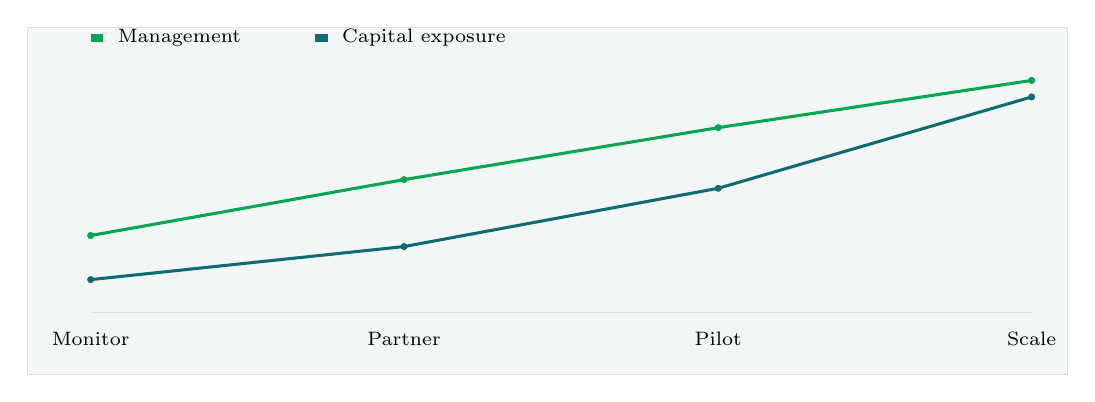
\begin{tikzpicture}[x=1cm,y=1cm]
\path[use as bounding box] (0,0) rectangle (13.20,4.40);
\fill[BOLight] (0,0) rectangle (13.20,4.40);
\draw[BOLine,line width=.35pt] (0,0) rectangle (13.20,4.40);
\draw[BOLine] (0.80,0.78) -- (12.75,0.78);
\draw[BOGreen,line width=1.1pt] (0.80,1.76) -- (4.78,2.47) -- (8.77,3.13) -- (12.75,3.73);
\fill[BOGreen] (0.80,1.76) circle (.045);
\fill[BOGreen] (4.78,2.47) circle (.045);
\fill[BOGreen] (8.77,3.13) circle (.045);
\fill[BOGreen] (12.75,3.73) circle (.045);
\draw[BOBlue,line width=1.1pt] (0.80,1.20) -- (4.78,1.62) -- (8.77,2.36) -- (12.75,3.52);
\fill[BOBlue] (0.80,1.20) circle (.045);
\fill[BOBlue] (4.78,1.62) circle (.045);
\fill[BOBlue] (8.77,2.36) circle (.045);
\fill[BOBlue] (12.75,3.52) circle (.045);
\node[anchor=north,align=center,text width=1.8cm] at (0.80,0.66) {\scriptsize Monitor};
\node[anchor=north,align=center,text width=1.8cm] at (4.78,0.66) {\scriptsize Partner};
\node[anchor=north,align=center,text width=1.8cm] at (8.77,0.66) {\scriptsize Pilot};
\node[anchor=north,align=center,text width=1.8cm] at (12.75,0.66) {\scriptsize Scale};
\fill[BOGreen] (0.80,4.22) rectangle (0.96,4.32);
\node[anchor=west] at (1.02,4.27) {\scriptsize Management};
\fill[BOBlue] (3.65,4.22) rectangle (3.81,4.32);
\node[anchor=west] at (3.87,4.27) {\scriptsize Capital exposure};
\end{tikzpicture}\par\vspace{2pt}
\vspace{1pt}\noindent\begin{minipage}[t]{0.56\linewidth}
{\footnotesize\color{BOText} Capital exposure should lag evidence maturity rather than lead it.}\par
\end{minipage}\hfill\begin{minipage}[t]{0.36\linewidth}
{\scriptsize\color{BOText}\begin{tabular}{p{31mm}>{\raggedleft\arraybackslash}p{18mm}}
\multicolumn{2}{l}{\textcolor{BOGreen}{\bfseries Visible readout}}\\[2pt]
Monitor & \textbf{40}\\[1pt]
Partner & \textbf{72}\\[1pt]
Pilot & \textbf{112}\\[1pt]
Scale & \textbf{162}\\[1pt]
\end{tabular}}\par
\end{minipage}\par\vspace{1pt}
\vspace{4pt}{\footnotesize\color{BOText} Capital exposure should lag evidence maturity rather than lead it.}\par
{\scriptsize\color{BOMuted} BlueOcean scenario synthesis.}\par

\clearpage
{\textcolor{BOGreen}{\scriptsize\bfseries EXHIBIT 3}}\par\vspace{4pt}
{\sffamily\fontsize{17}{21}\selectfont\color{BONavy} Key risks should be ranked by severity and manageability}\par
{\small\color{BOText} Risk exposure for Nuclear Fusion Commercialization Outlook and Strategic Implications}\par\vspace{6pt}
\noindent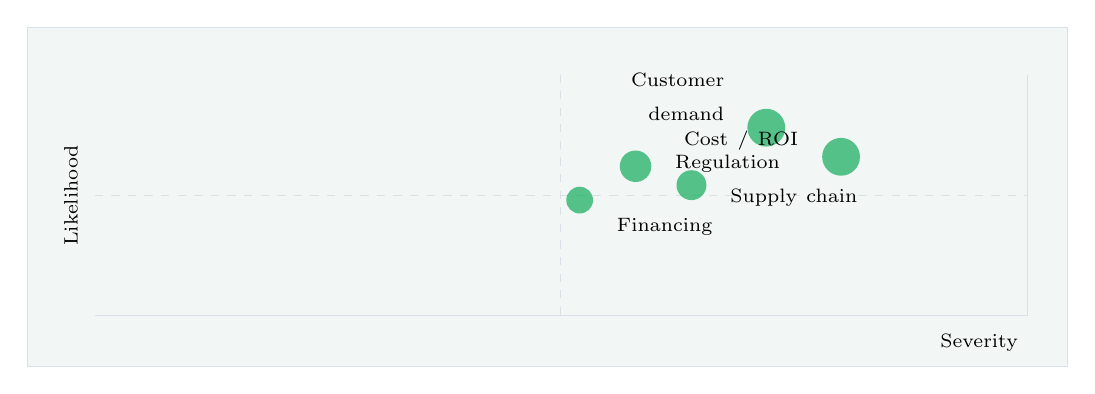
\begin{tikzpicture}[x=1cm,y=1cm]
\path[use as bounding box] (0,0) rectangle (13.20,4.30);
\fill[BOLight] (0,0) rectangle (13.20,4.30);
\draw[BOLine,line width=.35pt] (0,0) rectangle (13.20,4.30);
\draw[BOLine] (0.85,0.65) -- (12.70,0.65) -- (12.70,3.70);
\draw[BOLine,dashed] (0.85,2.17) -- (12.70,2.17);
\draw[BOLine,dashed] (6.77,0.65) -- (6.77,3.70);
\fill[BOGreen,opacity=.65] (9.38,3.03) circle (0.24);
\node[anchor=east,align=right,text width=2.10cm] at (8.97,3.42) {\scriptsize Customer demand};
\fill[BOGreen,opacity=.65] (10.33,2.66) circle (0.24);
\node[anchor=east,align=right,text width=2.10cm] at (9.91,2.87) {\scriptsize Cost / ROI};
\fill[BOGreen,opacity=.65] (7.72,2.54) circle (0.20);
\node[anchor=west,align=left,text width=2.10cm] at (8.10,2.57) {\scriptsize Regulation};
\fill[BOGreen,opacity=.65] (8.43,2.30) circle (0.19);
\node[anchor=west,align=left,text width=2.10cm] at (8.80,2.14) {\scriptsize Supply chain};
\fill[BOGreen,opacity=.65] (7.01,2.11) circle (0.17);
\node[anchor=west,align=left,text width=2.10cm] at (7.36,1.77) {\scriptsize Financing};
\node[anchor=north east] at (12.70,0.53) {\scriptsize Severity};
\node[anchor=center,rotate=90] at (0.55,2.17) {\scriptsize Likelihood};
\end{tikzpicture}\par\vspace{2pt}
\vspace{1pt}\noindent\begin{minipage}[t]{0.56\linewidth}
{\footnotesize\color{BOText} Bubble size indicates the management attention required.}\par
\end{minipage}\hfill\begin{minipage}[t]{0.36\linewidth}
{\scriptsize\color{BOText}\begin{tabular}{p{31mm}>{\raggedleft\arraybackslash}p{18mm}}
\multicolumn{2}{l}{\textcolor{BOGreen}{\bfseries Position}}\\[2pt]
Customer demand & \textbf{72 / 78}\\[1pt]
Cost / ROI & \textbf{80 / 66}\\[1pt]
Regulation & \textbf{58 / 62}\\[1pt]
Supply chain & \textbf{64 / 54}\\[1pt]
Financing & \textbf{52 / 48}\\[1pt]
\end{tabular}}\par
\end{minipage}\par\vspace{1pt}
\vspace{4pt}{\footnotesize\color{BOText} Bubble size indicates the management attention required.}\par
{\scriptsize\color{BOMuted} BlueOcean risk screen.}\par
\vspace{9pt}\textcolor{BOLine}{\rule{\linewidth}{0.3pt}}\vspace{8pt}
{\textcolor{BOGreen}{\scriptsize\bfseries EXHIBIT 4}}\par\vspace{4pt}
{\sffamily\fontsize{17}{21}\selectfont\color{BONavy} Diligence workload concentrates in customer, cost and policy proof}\par
{\small\color{BOText} Near-term validation load for Nuclear Fusion Commercialization Outlook and Strategic Implications}\par\vspace{6pt}
\noindent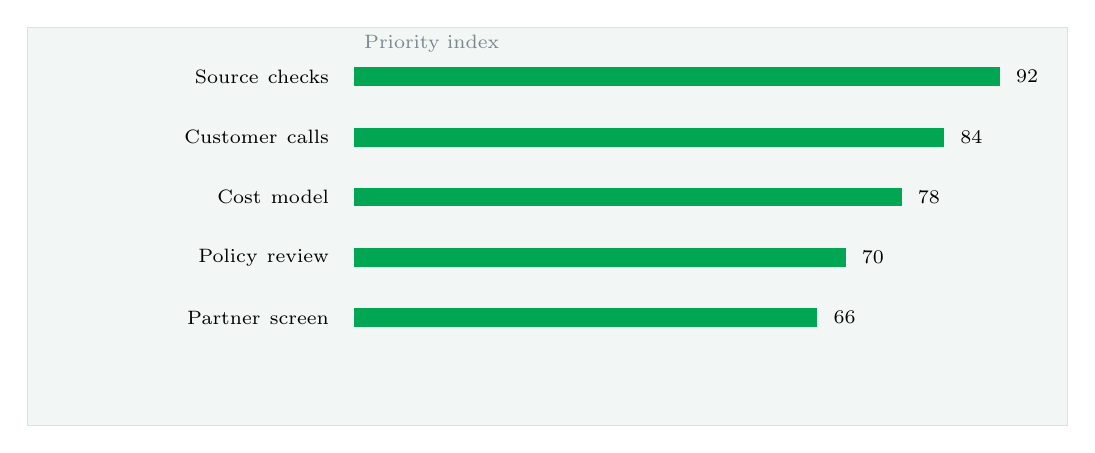
\begin{tikzpicture}[x=1cm,y=1cm]
\path[use as bounding box] (0,0) rectangle (13.20,5.05);
\fill[BOLight] (0,0) rectangle (13.20,5.05);
\draw[BOLine,line width=.35pt] (0,0) rectangle (13.20,5.05);
\node[anchor=west] at (4.15,4.85) {\scriptsize\color{BOMuted} Priority index};
\node[anchor=east,align=right,text width=3.93cm] at (3.95,4.43) {\scriptsize Source checks};
\fill[BOLight] (4.15,4.31) rectangle (12.35,4.55);
\fill[BOGreen] (4.15,4.31) rectangle (12.35,4.55);
\node[anchor=west] at (12.43,4.43) {\scriptsize 92};
\node[anchor=east,align=right,text width=3.93cm] at (3.95,3.66) {\scriptsize Customer calls};
\fill[BOLight] (4.15,3.54) rectangle (12.35,3.78);
\fill[BOGreen] (4.15,3.54) rectangle (11.64,3.78);
\node[anchor=west] at (11.72,3.66) {\scriptsize 84};
\node[anchor=east,align=right,text width=3.93cm] at (3.95,2.90) {\scriptsize Cost model};
\fill[BOLight] (4.15,2.78) rectangle (12.35,3.02);
\fill[BOGreen] (4.15,2.78) rectangle (11.10,3.02);
\node[anchor=west] at (11.18,2.90) {\scriptsize 78};
\node[anchor=east,align=right,text width=3.93cm] at (3.95,2.13) {\scriptsize Policy review};
\fill[BOLight] (4.15,2.01) rectangle (12.35,2.25);
\fill[BOGreen] (4.15,2.01) rectangle (10.39,2.25);
\node[anchor=west] at (10.47,2.13) {\scriptsize 70};
\node[anchor=east,align=right,text width=3.93cm] at (3.95,1.37) {\scriptsize Partner screen};
\fill[BOLight] (4.15,1.25) rectangle (12.35,1.49);
\fill[BOGreen] (4.15,1.25) rectangle (10.03,1.49);
\node[anchor=west] at (10.11,1.37) {\scriptsize 66};
\end{tikzpicture}\par\vspace{2pt}
\vspace{1pt}\noindent\begin{minipage}[t]{0.56\linewidth}
{\footnotesize\color{BOText} The most valuable work closes open questions that can change the decision.}\par
\end{minipage}\hfill\begin{minipage}[t]{0.36\linewidth}
{\scriptsize\color{BOText}\begin{tabular}{p{31mm}>{\raggedleft\arraybackslash}p{18mm}}
\multicolumn{2}{l}{\textcolor{BOGreen}{\bfseries Visible readout}}\\[2pt]
Source checks & \textbf{92}\\[1pt]
Customer calls & \textbf{84}\\[1pt]
Cost model & \textbf{78}\\[1pt]
Policy review & \textbf{70}\\[1pt]
Partner screen & \textbf{66}\\[1pt]
\end{tabular}}\par
\end{minipage}\par\vspace{1pt}
\vspace{4pt}{\footnotesize\color{BOText} The most valuable work closes open questions that can change the decision.}\par
{\scriptsize\color{BOMuted} BlueOcean public-source synthesis.}\par

\clearpage
\label{chap:1}
\noindent\begin{tikzpicture}
\path[use as bounding box] (0,0) rectangle (\linewidth,54mm);
\clip (0,0) rectangle (\linewidth,54mm);
\node[anchor=north west,inner sep=0] at (0,54mm) {
\includegraphics[width=\linewidth]{assets/image-1.png}};
\end{tikzpicture}
\vspace{0pt}
\noindent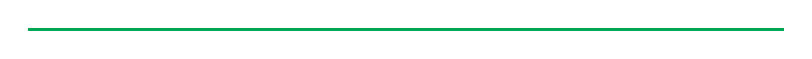
\begin{tikzpicture}
\fill[BOGreen] (0,0) rectangle (96mm,1.2pt);
\end{tikzpicture}\par\vspace{8pt}
{\Large\sffamily\bfseries\color{BONavy} Nuclear Fusion Is Approaching Technical Viability but Commercial Deployment Remains Over a Decade Away}\par\vspace{4pt}
{\sffamily\fontsize{15}{20}\selectfont\color{BOGreen} Fusion\BOApos{}s scientific feasibility has been proven, but the path to commercial power plants is long and uncertain, requiring patient capital and milestone-based investment.}\par\vspace{9pt}
\begin{multicols}{2}
{\small Nuclear fusion has long been hailed as the holy grail of clean energy. The promise is immense: virtually limitless fuel, no carbon emissions, and minimal long-lived radioactive waste. After decades of research, the field is experiencing a renaissance, driven by scientific breakthroughs and a surge of private investment. However, the path from laboratory experiments to commercial power plants is fraught with technical, regulatory, and market challenges.}\par
{\small The most significant recent milestone was achieved in December 2022 at Lawrence Livermore National Laboratory, where the National Ignition Facility (NIF) demonstrated fusion ignition-producing more energy from fusion than the laser energy used to drive it. This was a historic scientific achievement, but it was a single experiment under controlled conditions, not a sustained power source. The NIF is a research facility, not a prototype power plant.}\par
{\small The leading approach to fusion remains magnetic confinement, particularly the tokamak design. The international ITER project in France is the largest tokamak ever built, aiming to demonstrate sustained fusion power at scale. ITER has been under construction since 2013 and has faced repeated delays. The current timeline expects first plasma in 2025-2027 and full fusion power in the 2030s. ITER is not designed to produce electricity; it is an experimental step toward a demonstration power plant.}\par
{\small Private companies are pursuing faster timelines. Commonwealth Fusion Systems (CFS), a spinout from MIT, is building SPARC, a compact tokamak using high-temperature superconducting magnets. CFS aims to demonstrate net energy gain by 2025-2026 and build a commercial pilot plant, ARC, by the early 2030s. Other notable private ventures include Helion Energy, which is developing a field-reversed configuration design and has secured offtake agreements with Microsoft, and TAE Technologies, which uses a field-reversed configuration with neutral beam injection.}\par
{\small Despite the optimism, no private company has yet demonstrated net energy gain in a reactor-relevant configuration. The claims of commercial reactors by 2030 remain unverified and are considered optimistic by most experts. The Fusion Industry Association reports that over \$6 billion has been invested in private fusion since 2015, but the industry is still in the early stages of technology development.}\par
{\small The timeline to commercial fusion is best understood in phases. The current decade (2020s) is focused on demonstrating scientific feasibility and engineering scale-up. The 2030s will likely see the first pilot plants, if milestones are met. Commercial deployment, if successful, is unlikely before 2040-2050. This long horizon means fusion will not disrupt energy markets in the near term, but it could become a critical baseload clean power source in the second half of the century.}\par
{\small The immediate management question is not whether the opportunity is exciting; it is whether budget, partner access or management attention should be committed now. Low-cost validation can start early, while larger capital commitments should wait for customer, cost, financing, regulatory or operating proof.}\par
{\small The current source base is useful but incomplete. Retained source signal: gov/science/fusion-energy-sciences/fusion-milestone-based-development-program Search context: nuclear fusion commercialization timeline 2025 The page body could not be fully extracted, so this source should be treated as a lower-confidence. A quarterly review rhythm is more useful than a one-time verdict because the facts that matter will change as customers, regulators and suppliers move.}\par
\end{multicols}
\vspace{5pt}\noindent\begin{tabularx}{\linewidth}{Y Y Y}
{\textcolor{BOGreen}{\bfseries 01}}\par{\scriptsize\color{BOText} Fusion is scientifically feasible but commercially distant (likely post-2040)} & {\textcolor{BOGreen}{\bfseries 02}}\par{\scriptsize\color{BOText} Private companies offer faster timelines but remain unverified} & {\textcolor{BOGreen}{\bfseries 03}}\par{\scriptsize\color{BOText} Invest now for optionality, not near-term returns} \\
\end{tabularx}\par\vspace{2pt}
\label{chap:1:end}

\clearpage
{\textcolor{BOGreen}{\scriptsize\bfseries EXHIBIT 5}}\par\vspace{4pt}
{\sffamily\fontsize{17}{21}\selectfont\color{BONavy} Scenario choices should compare attractiveness with readiness}\par
{\small\color{BOText} Strategic option comparison for Nuclear Fusion Commercialization Outlook and Strategic Implications}\par\vspace{6pt}
\noindent\fcolorbox{BOLine}{BOLight}{\begin{minipage}{0.96\linewidth}\vspace{4pt}{\scriptsize\begin{tabular}{p{38mm}>{\centering\arraybackslash}p{21mm}>{\centering\arraybackslash}p{21mm}>{\centering\arraybackslash}p{21mm}>{\centering\arraybackslash}p{21mm}}
 & {\bfseries Attractiveness} & {\bfseries Readiness} & {\bfseries Confidence} & {\bfseries Capital need} \\
\hline
{\bfseries Nuclear Fusion Is Approaching} & \colorbox{BOGreen}{\textcolor{white}{\strut\hspace{5pt}5\hspace{5pt}}} & \colorbox{BOBlue}{\textcolor{white}{\strut\hspace{5pt}3\hspace{5pt}}} & \colorbox{BOLight}{\textcolor{BOText}{\strut\hspace{5pt}2\hspace{5pt}}} & \colorbox{BOLight}{\textcolor{BOText}{\strut\hspace{5pt}2\hspace{5pt}}} \\
{\bfseries Magnetic Confinement Leads} & \colorbox{BOGreen}{\textcolor{white}{\strut\hspace{5pt}4\hspace{5pt}}} & \colorbox{BOGreen}{\textcolor{white}{\strut\hspace{5pt}4\hspace{5pt}}} & \colorbox{BOBlue}{\textcolor{white}{\strut\hspace{5pt}3\hspace{5pt}}} & \colorbox{BOBlue}{\textcolor{white}{\strut\hspace{5pt}3\hspace{5pt}}} \\
{\bfseries Private Fusion Companies Are} & \colorbox{BOGreen}{\textcolor{white}{\strut\hspace{5pt}4\hspace{5pt}}} & \colorbox{BOLight}{\textcolor{BOText}{\strut\hspace{5pt}2\hspace{5pt}}} & \colorbox{BOLight}{\textcolor{BOText}{\strut\hspace{5pt}2\hspace{5pt}}} & \colorbox{BOGreen}{\textcolor{white}{\strut\hspace{5pt}4\hspace{5pt}}} \\
{\bfseries Regulatory and Licensing} & \colorbox{BOBlue}{\textcolor{white}{\strut\hspace{5pt}3\hspace{5pt}}} & \colorbox{BOBlue}{\textcolor{white}{\strut\hspace{5pt}3\hspace{5pt}}} & \colorbox{BOBlue}{\textcolor{white}{\strut\hspace{5pt}3\hspace{5pt}}} & \colorbox{BOLight}{\textcolor{BOText}{\strut\hspace{5pt}2\hspace{5pt}}} \\
{\bfseries Fusion\BOApos{}s Strategic Value Lies} & \colorbox{BOGreen}{\textcolor{white}{\strut\hspace{5pt}5\hspace{5pt}}} & \colorbox{BOBlue}{\textcolor{white}{\strut\hspace{5pt}3\hspace{5pt}}} & \colorbox{BOBlue}{\textcolor{white}{\strut\hspace{5pt}3\hspace{5pt}}} & \colorbox{BOBlue}{\textcolor{white}{\strut\hspace{5pt}3\hspace{5pt}}} \\
\end{tabular}}\vspace{4pt}\end{minipage}}\par\vspace{2pt}
\vspace{1pt}\noindent\begin{minipage}[t]{0.56\linewidth}
{\footnotesize\color{BOText} The matrix ranks where the next validation work should focus.}\par
\end{minipage}\hfill\begin{minipage}[t]{0.36\linewidth}
{\scriptsize\color{BOText}\begin{tabular}{p{31mm}>{\raggedleft\arraybackslash}p{18mm}}
\multicolumn{2}{l}{\textcolor{BOGreen}{\bfseries Matrix readout}}\\[2pt]
Nuclear Fusion Is & \textbf{5 / 3}\\[1pt]
Magnetic Confinement & \textbf{4 / 4}\\[1pt]
Private Fusion & \textbf{4 / 2}\\[1pt]
Regulatory & \textbf{3 / 3}\\[1pt]
\end{tabular}}\par
\end{minipage}\par\vspace{1pt}
\vspace{4pt}{\footnotesize\color{BOText} The matrix ranks where the next validation work should focus.}\par
{\scriptsize\color{BOMuted} BlueOcean qualitative assessment.}\par
\vspace{9pt}\textcolor{BOLine}{\rule{\linewidth}{0.3pt}}\vspace{8pt}
{\textcolor{BOGreen}{\scriptsize\bfseries EXHIBIT 6}}\par\vspace{4pt}
{\sffamily\fontsize{17}{21}\selectfont\color{BONavy} Validation effort shifts from customer proof to policy and partners}\par
{\small\color{BOText} Quarterly validation mix for Nuclear Fusion Commercialization Outlook and Strategic Implications}\par\vspace{6pt}
\noindent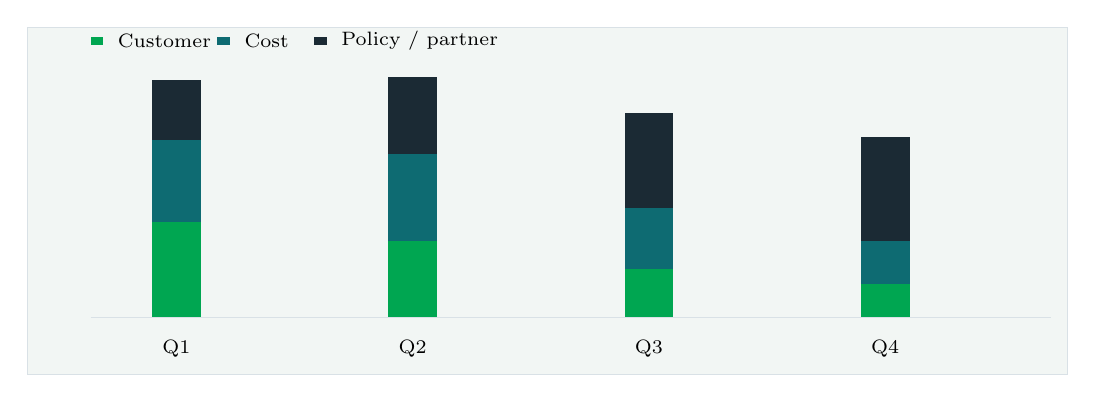
\begin{tikzpicture}[x=1cm,y=1cm]
\path[use as bounding box] (0,0) rectangle (13.20,4.40);
\fill[BOLight] (0,0) rectangle (13.20,4.40);
\draw[BOLine,line width=.35pt] (0,0) rectangle (13.20,4.40);
\draw[BOLine] (0.80,0.72) -- (13.00,0.72);
\fill[BOGreen] (1.58,0.72) rectangle (2.20,1.93);
\fill[BOBlue] (1.58,1.93) rectangle (2.20,2.97);
\fill[BONavy] (1.58,2.97) rectangle (2.20,3.74);
\node[anchor=north,align=center,text width=2.76cm] at (1.89,0.55) {\scriptsize Q1};
\fill[BOGreen] (4.58,0.72) rectangle (5.20,1.69);
\fill[BOBlue] (4.58,1.69) rectangle (5.20,2.80);
\fill[BONavy] (4.58,2.80) rectangle (5.20,3.77);
\node[anchor=north,align=center,text width=2.76cm] at (4.89,0.55) {\scriptsize Q2};
\fill[BOGreen] (7.58,0.72) rectangle (8.20,1.34);
\fill[BOBlue] (7.58,1.34) rectangle (8.20,2.11);
\fill[BONavy] (7.58,2.11) rectangle (8.20,3.32);
\node[anchor=north,align=center,text width=2.76cm] at (7.89,0.55) {\scriptsize Q3};
\fill[BOGreen] (10.58,0.72) rectangle (11.20,1.14);
\fill[BOBlue] (10.58,1.14) rectangle (11.20,1.69);
\fill[BONavy] (10.58,1.69) rectangle (11.20,3.01);
\node[anchor=north,align=center,text width=2.76cm] at (10.89,0.55) {\scriptsize Q4};
\fill[BOGreen] (0.80,4.18) rectangle (0.96,4.28);
\node[anchor=west] at (1.02,4.23) {\scriptsize Customer};
\fill[BOBlue] (2.41,4.18) rectangle (2.57,4.28);
\node[anchor=west] at (2.63,4.23) {\scriptsize Cost};
\fill[BONavy] (3.64,4.18) rectangle (3.80,4.28);
\node[anchor=west] at (3.86,4.23) {\scriptsize Policy / partner};
\end{tikzpicture}\par\vspace{2pt}
\vspace{1pt}\noindent\begin{minipage}[t]{0.56\linewidth}
{\footnotesize\color{BOText} The validation cadence should improve facts before escalating resource commitment.}\par
\end{minipage}\hfill\begin{minipage}[t]{0.36\linewidth}
{\scriptsize\color{BOText}\begin{tabular}{p{31mm}>{\raggedleft\arraybackslash}p{18mm}}
\multicolumn{2}{l}{\textcolor{BOGreen}{\bfseries Visible readout}}\\[2pt]
Q1 & \textbf{87}\\[1pt]
Q2 & \textbf{88}\\[1pt]
Q3 & \textbf{75}\\[1pt]
Q4 & \textbf{66}\\[1pt]
\end{tabular}}\par
\end{minipage}\par\vspace{1pt}
\vspace{4pt}{\footnotesize\color{BOText} The validation cadence should improve facts before escalating resource commitment.}\par
{\scriptsize\color{BOMuted} BlueOcean public-source synthesis.}\par

\clearpage
\label{chap:2}
\noindent\begin{tikzpicture}
\path[use as bounding box] (0,0) rectangle (\linewidth,54mm);
\clip (0,0) rectangle (\linewidth,54mm);
\node[anchor=north west,inner sep=0] at (0,54mm) {
\includegraphics[width=\linewidth]{assets/image-2.png}};
\end{tikzpicture}
\vspace{0pt}
\noindent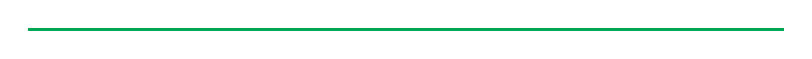
\begin{tikzpicture}
\fill[BOGreen] (0,0) rectangle (96mm,1.2pt);
\end{tikzpicture}\par\vspace{8pt}
{\Large\sffamily\bfseries\color{BONavy} Magnetic Confinement Leads in Maturity but Faces High Capital Costs and Long Construction Times}\par\vspace{4pt}
{\sffamily\fontsize{15}{20}\selectfont\color{BOGreen} Magnetic confinement, especially tokamaks, is the most proven approach but requires large capital and long lead times, making it suitable for patient investors with deep pockets.}\par\vspace{9pt}
\begin{multicols}{2}
{\small Magnetic confinement fusion, particularly the tokamak design, is the most mature and well-funded approach. The underlying physics is well understood, and large experiments like JET (Joint European Torus) have achieved significant milestones, including producing 16 MW of fusion power in 1997. However, scaling up to a commercial reactor presents enormous engineering challenges.}\par
{\small The ITER project is the flagship of magnetic confinement. With a budget exceeding \$20 billion and participation from 35 countries, ITER is designed to produce 500 MW of fusion power from 50 MW of input, a Q value of 10. ITER\BOApos{}s construction has been plagued by delays and cost overruns, partly due to the complexity of coordinating international partners and the challenges of manufacturing large-scale components.}\par
{\small The operating takeaway is that private companies are attempting to leapfrog ITER by using advanced technologies. Commonwealth Fusion Systems\BOApos{} SPARC tokamak will be much smaller than ITER but aims to achieve Q>2 using high-temperature superconducting (HTS) magnets. HTS magnets operate at higher temperatures and magnetic fields, allowing for more compact and potentially cheaper reactors. CFS has raised over \$2 billion and is building SPARC in Devens, Massachusetts.}\par
{\small Another magnetic confinement variant is the stellarator, which uses twisted magnetic fields to confine plasma without the need for a plasma current. Stellarators are inherently steady-state and avoid some instabilities of tokamaks, but they are more complex to design and build. The Wendelstein 7-X in Germany is the largest stellarator and has demonstrated good plasma confinement, but it is not designed for fusion power.}\par
{\small The capital costs of magnetic confinement reactors are a major barrier. ITER\BOApos{}s cost is not representative of a commercial plant, but it highlights the scale of investment required. Private companies claim they can build reactors for \$1-3 billion, but these estimates are unverified. The levelized cost of electricity (LCOE) from fusion is projected to be \$50-100 per MWh, but this depends on achieving high availability and low fuel costs.}\par
{\small Construction timelines for magnetic confinement are long. ITER has taken over a decade to build, and even compact designs like SPARC are expected to take 5-7 years from groundbreaking to operation. Commercial plants would likely take similar or longer times, especially given the need for regulatory approvals and supply chain development.}\par
{\small The supply chain for fusion components is immature. Key materials like tritium (the fusion fuel) are scarce and must be bred within the reactor. Beryllium, used in plasma-facing components, is toxic and expensive. High-temperature superconductors are still produced in limited quantities. These bottlenecks could delay deployment and increase costs.}\par
{\small Despite these challenges, magnetic confinement remains the most credible path to fusion power. The combination of public projects like ITER and private ventures like CFS provides a diversified approach. Investors should monitor milestones such as SPARC\BOApos{}s first plasma and ITER\BOApos{}s first fusion power to gauge progress.}\par
\end{multicols}
\vspace{5pt}\noindent\begin{tabularx}{\linewidth}{Y Y Y}
{\textcolor{BOGreen}{\bfseries 01}}\par{\scriptsize\color{BOText} Tokamaks are most mature but capital-intensive} & {\textcolor{BOGreen}{\bfseries 02}}\par{\scriptsize\color{BOText} Private compact tokamaks (e.g., SPARC) could reduce costs and timelines} & {\textcolor{BOGreen}{\bfseries 03}}\par{\scriptsize\color{BOText} Supply chain bottlenecks for tritium and HTS magnets are key risks} \\
\end{tabularx}\par\vspace{2pt}
\label{chap:2:end}

\clearpage
{\textcolor{BOGreen}{\scriptsize\bfseries EXHIBIT 7}}\par\vspace{4pt}
{\sffamily\fontsize{17}{21}\selectfont\color{BONavy} Cost structure must be decomposed before underwriting}\par
{\small\color{BOText} Cost diligence view for Nuclear Fusion Commercialization Outlook and Strategic Implications}\par\vspace{6pt}
\noindent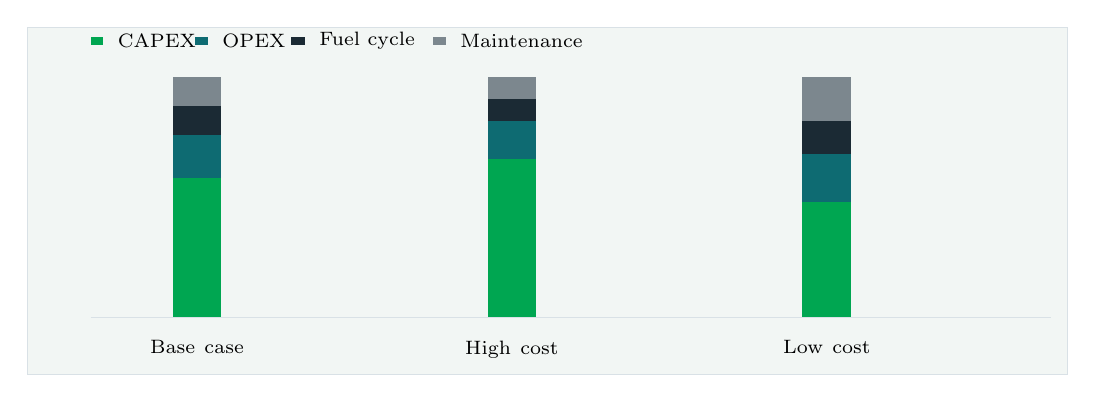
\begin{tikzpicture}[x=1cm,y=1cm]
\path[use as bounding box] (0,0) rectangle (13.20,4.40);
\fill[BOLight] (0,0) rectangle (13.20,4.40);
\draw[BOLine,line width=.35pt] (0,0) rectangle (13.20,4.40);
\draw[BOLine] (0.80,0.72) -- (13.00,0.72);
\fill[BOGreen] (1.84,0.72) rectangle (2.46,2.49);
\fill[BOBlue] (1.84,2.49) rectangle (2.46,3.04);
\fill[BONavy] (1.84,3.04) rectangle (2.46,3.40);
\fill[BOMuted] (1.84,3.40) rectangle (2.46,3.77);
\node[anchor=north,align=center,text width=3.68cm] at (2.15,0.55) {\scriptsize Base case};
\fill[BOGreen] (5.84,0.72) rectangle (6.46,2.73);
\fill[BOBlue] (5.84,2.73) rectangle (6.46,3.22);
\fill[BONavy] (5.84,3.22) rectangle (6.46,3.50);
\fill[BOMuted] (5.84,3.50) rectangle (6.46,3.77);
\node[anchor=north,align=center,text width=3.68cm] at (6.15,0.55) {\scriptsize High cost};
\fill[BOGreen] (9.84,0.72) rectangle (10.46,2.18);
\fill[BOBlue] (9.84,2.18) rectangle (10.46,2.79);
\fill[BONavy] (9.84,2.79) rectangle (10.46,3.22);
\fill[BOMuted] (9.84,3.22) rectangle (10.46,3.77);
\node[anchor=north,align=center,text width=3.68cm] at (10.15,0.55) {\scriptsize Low cost};
\fill[BOGreen] (0.80,4.18) rectangle (0.96,4.28);
\node[anchor=west] at (1.02,4.23) {\scriptsize CAPEX};
\fill[BOBlue] (2.12,4.18) rectangle (2.29,4.28);
\node[anchor=west] at (2.35,4.23) {\scriptsize OPEX};
\fill[BONavy] (3.35,4.18) rectangle (3.52,4.28);
\node[anchor=west] at (3.58,4.23) {\scriptsize Fuel cycle};
\fill[BOMuted] (5.15,4.18) rectangle (5.31,4.28);
\node[anchor=west] at (5.37,4.23) {\scriptsize Maintenance};
\end{tikzpicture}\par\vspace{2pt}
\vspace{1pt}\noindent\begin{minipage}[t]{0.56\linewidth}
{\footnotesize\color{BOText} The chart separates capital, operating and maintenance drivers so management can test which cost lever would change the investment case.}\par
\end{minipage}\hfill\begin{minipage}[t]{0.36\linewidth}
{\scriptsize\color{BOText}\begin{tabular}{p{31mm}>{\raggedleft\arraybackslash}p{18mm}}
\multicolumn{2}{l}{\textcolor{BOGreen}{\bfseries Visible readout}}\\[2pt]
Base case & \textbf{100}\\[1pt]
High cost & \textbf{100}\\[1pt]
Low cost & \textbf{100}\\[1pt]
\end{tabular}}\par
\end{minipage}\par\vspace{1pt}
\vspace{4pt}{\footnotesize\color{BOText} The chart separates capital, operating and maintenance drivers so management can test which cost lever would change the investment case.}\par
{\scriptsize\color{BOMuted} BlueOcean public-source synthesis.}\par
\vspace{9pt}\textcolor{BOLine}{\rule{\linewidth}{0.3pt}}\vspace{8pt}
{\textcolor{BOGreen}{\scriptsize\bfseries EXHIBIT 8}}\par\vspace{4pt}
{\sffamily\fontsize{17}{21}\selectfont\color{BONavy} Timeline confidence falls as milestones move from lab to grid}\par
{\small\color{BOText} Milestone confidence for Nuclear Fusion Commercialization Outlook and Strategic Implications}\par\vspace{6pt}
\noindent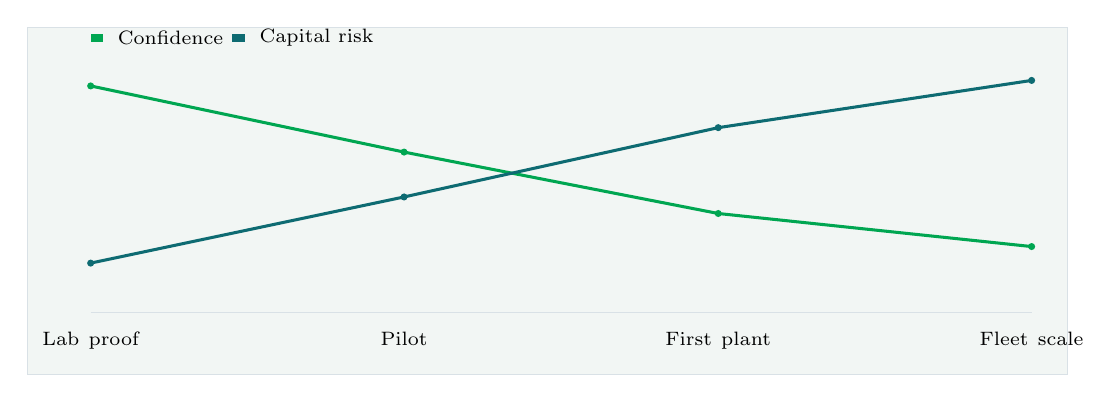
\begin{tikzpicture}[x=1cm,y=1cm]
\path[use as bounding box] (0,0) rectangle (13.20,4.40);
\fill[BOLight] (0,0) rectangle (13.20,4.40);
\draw[BOLine,line width=.35pt] (0,0) rectangle (13.20,4.40);
\draw[BOLine] (0.80,0.78) -- (12.75,0.78);
\draw[BOGreen,line width=1.1pt] (0.80,3.66) -- (4.78,2.82) -- (8.77,2.04) -- (12.75,1.62);
\fill[BOGreen] (0.80,3.66) circle (.045);
\fill[BOGreen] (4.78,2.82) circle (.045);
\fill[BOGreen] (8.77,2.04) circle (.045);
\fill[BOGreen] (12.75,1.62) circle (.045);
\draw[BOBlue,line width=1.1pt] (0.80,1.41) -- (4.78,2.25) -- (8.77,3.13) -- (12.75,3.73);
\fill[BOBlue] (0.80,1.41) circle (.045);
\fill[BOBlue] (4.78,2.25) circle (.045);
\fill[BOBlue] (8.77,3.13) circle (.045);
\fill[BOBlue] (12.75,3.73) circle (.045);
\node[anchor=north,align=center,text width=1.8cm] at (0.80,0.66) {\scriptsize Lab proof};
\node[anchor=north,align=center,text width=1.8cm] at (4.78,0.66) {\scriptsize Pilot};
\node[anchor=north,align=center,text width=1.8cm] at (8.77,0.66) {\scriptsize First plant};
\node[anchor=north,align=center,text width=1.8cm] at (12.75,0.66) {\scriptsize Fleet scale};
\fill[BOGreen] (0.80,4.22) rectangle (0.96,4.32);
\node[anchor=west] at (1.02,4.27) {\scriptsize Confidence};
\fill[BOBlue] (2.60,4.22) rectangle (2.76,4.32);
\node[anchor=west] at (2.82,4.27) {\scriptsize Capital risk};
\end{tikzpicture}\par\vspace{2pt}
\vspace{1pt}\noindent\begin{minipage}[t]{0.56\linewidth}
{\footnotesize\color{BOText} Decision confidence should be staged by milestone maturity.}\par
\end{minipage}\hfill\begin{minipage}[t]{0.36\linewidth}
{\scriptsize\color{BOText}\begin{tabular}{p{31mm}>{\raggedleft\arraybackslash}p{18mm}}
\multicolumn{2}{l}{\textcolor{BOGreen}{\bfseries Visible readout}}\\[2pt]
Lab proof & \textbf{100}\\[1pt]
Pilot & \textbf{100}\\[1pt]
First plant & \textbf{103}\\[1pt]
Fleet scale & \textbf{108}\\[1pt]
\end{tabular}}\par
\end{minipage}\par\vspace{1pt}
\vspace{4pt}{\footnotesize\color{BOText} Decision confidence should be staged by milestone maturity.}\par
{\scriptsize\color{BOMuted} BlueOcean milestone assessment.}\par

\clearpage
\label{chap:3}
\noindent\begin{tikzpicture}
\path[use as bounding box] (0,0) rectangle (\linewidth,54mm);
\clip (0,0) rectangle (\linewidth,54mm);
\node[anchor=north west,inner sep=0] at (0,54mm) {
\includegraphics[width=\linewidth]{assets/image-3.png}};
\end{tikzpicture}
\vspace{0pt}
\noindent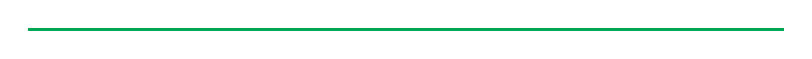
\begin{tikzpicture}
\fill[BOGreen] (0,0) rectangle (96mm,1.2pt);
\end{tikzpicture}\par\vspace{8pt}
{\Large\sffamily\bfseries\color{BONavy} Private Fusion Companies Are Accelerating Timelines with Innovative Designs and Substantial Funding}\par\vspace{4pt}
{\sffamily\fontsize{15}{20}\selectfont\color{BOGreen} Private fusion ventures have attracted over \$6 billion and promise faster commercialization, but their technical claims remain unproven, requiring rigorous due diligence.}\par\vspace{9pt}
\begin{multicols}{2}
{\small The fusion landscape has been transformed by the entry of private companies. Since 2015, over \$6 billion has been invested in private fusion ventures, according to the Fusion Industry Association. These companies are pursuing a variety of approaches, from compact tokamaks to aneutronic fusion, and many claim they can achieve commercial fusion faster than traditional government projects.}\par
{\small Commonwealth Fusion Systems (CFS) is the best-funded private fusion company, with over \$2 billion in funding. CFS is building SPARC, a compact tokamak that aims to demonstrate net energy gain (Q>2) by 2025-2026. SPARC uses high-temperature superconducting (HTS) magnets, which are a key enabling technology. If successful, CFS plans to build a commercial pilot plant, ARC, by the early 2030s.}\par
{\small Helion Energy is developing a field-reversed configuration (FRC) reactor that uses a pulsed approach to directly capture electricity without a steam turbine. Helion has raised over \$600 million and signed a power purchase agreement with Microsoft, aiming to deliver electricity by 2028. However, Helion has not yet demonstrated net energy gain, and its timeline is considered aggressive.}\par
{\small TAE Technologies uses a field-reversed configuration with neutral beam injection to heat plasma. TAE has raised over \$1 billion and operates a large experimental device, Norman. The company aims to demonstrate net energy gain by 2025-2026 and build a commercial plant by 2030. TAE\BOApos{}s approach uses hydrogen-boron fuel, which is aneutronic and produces fewer neutrons, reducing activation and waste.}\par
{\small Other notable companies include General Fusion, which uses a magnetized target fusion approach with a liquid metal liner, and Zap Energy, which uses a Z-pinch design. Each approach has its own technical challenges and timelines. The diversity of approaches is a strength, as it increases the chances that at least one will succeed, but it also complicates investment decisions.}\par
{\small The funding landscape for private fusion has been robust, but there are signs of cooling. After a peak in 2022, investment levels have declined in 2024, partly due to macroeconomic conditions and the lack of near-term milestones. Companies that fail to demonstrate progress may struggle to secure follow-on funding.}\par
{\small For investors, the key is to conduct deep technical due diligence. Look for companies with credible physics, experienced teams, and clear milestones. Avoid those that rely on unproven physics or overly optimistic timelines. A portfolio approach across multiple designs and stages of development can mitigate risk.}\par
{\small Every opportunity eventually returns to cost, revenue, margin, cash flow and timing. If sourced evidence does not support market size, ROI, unit economics or share, those items should remain explicit assumptions rather than conclusions.}\par
\end{multicols}
\vspace{5pt}\noindent\begin{tabularx}{\linewidth}{Y Y Y}
{\textcolor{BOGreen}{\bfseries 01}}\par{\scriptsize\color{BOText} Over \$6 billion invested in private fusion since 2015} & {\textcolor{BOGreen}{\bfseries 02}}\par{\scriptsize\color{BOText} Diverse approaches: tokamaks, FRC, Z-pinch, etc} & {\textcolor{BOGreen}{\bfseries 03}}\par{\scriptsize\color{BOText} Due diligence must focus on technical milestones, not hype} \\
\end{tabularx}\par\vspace{2pt}
\label{chap:3:end}

\clearpage
\label{chap:4}
\noindent\begin{tikzpicture}
\path[use as bounding box] (0,0) rectangle (\linewidth,54mm);
\clip (0,0) rectangle (\linewidth,54mm);
\node[anchor=north west,inner sep=0] at (0,54mm) {
\includegraphics[width=\linewidth]{assets/image-4.png}};
\end{tikzpicture}
\vspace{0pt}
\noindent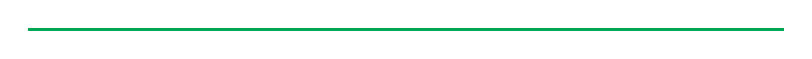
\begin{tikzpicture}
\fill[BOGreen] (0,0) rectangle (96mm,1.2pt);
\end{tikzpicture}\par\vspace{8pt}
{\Large\sffamily\bfseries\color{BONavy} Regulatory and Licensing Frameworks Are Underdeveloped, Posing Significant Timeline Risks}\par\vspace{4pt}
{\sffamily\fontsize{15}{20}\selectfont\color{BOGreen} Fusion reactors lack a clear regulatory pathway, which could delay deployment by years. Early engagement with regulators is critical to shaping the rules.}\par\vspace{9pt}
\begin{multicols}{2}
{\small One of the most significant non-technical barriers to fusion commercialization is the lack of a regulatory and licensing framework. Fusion reactors are not fission reactors, but they share some characteristics, such as the use of radioactive materials (tritium) and the potential for accidents. However, fusion has fundamentally different safety profiles: it cannot sustain a runaway chain reaction, and the radioactive waste is much shorter-lived.}\par
{\small In the United States, the Nuclear Regulatory Commission (NRC) has not yet established a licensing framework for fusion reactors. The NRC is currently studying the issue and has indicated that fusion may be regulated under a different framework than fission, but the timeline for rulemaking is uncertain. The National Academies study \BOApos{}Bringing Fusion to the U.S. Grid\BOApos{} highlights this as a critical gap and recommends that the NRC develop fusion-specific regulations by 2028.}\par
{\small Other countries are also grappling with fusion regulation. The United Kingdom has established a fusion regulatory framework under the Health and Safety Executive, which treats fusion as a nuclear facility but with tailored requirements. Canada and Japan are also developing frameworks. The lack of harmonization across countries could complicate international projects and supply chains.}\par
{\small The regulatory uncertainty creates risks for investors and developers. Without clear rules, it is difficult to estimate the cost and timeline for licensing a fusion plant. Early engagement with regulators is essential to shape the rules and ensure they are science-based and proportionate to the risks.}\par
{\small Industry consortia, such as the Fusion Industry Association, are advocating for risk-informed, performance-based regulations that recognize the inherent safety of fusion. They argue that fusion should not be subject to the same stringent requirements as fission, which could make it economically unviable.}\par
{\small For companies planning to build fusion plants, the regulatory pathway should be a key consideration in site selection. Some countries may offer more favorable regulatory environments, at least initially. The first-mover advantage in licensing could be significant.}\par
{\small The timeline for regulatory development is uncertain. The NRC\BOApos{}s process typically takes several years, and fusion-specific rules may not be in place until the late 2020s or early 2030s. This could delay the construction of first-of-a-kind plants, as developers may need to wait for clarity before committing to large capital expenditures.}\par
{\small In the meantime, some companies are pursuing alternative strategies, such as building fusion plants in countries with existing frameworks (e.g., the UK) or using a phased approach that starts with smaller, non-power applications that may face less regulatory scrutiny.}\par
\end{multicols}
\vspace{5pt}\noindent\begin{tabularx}{\linewidth}{Y Y Y}
{\textcolor{BOGreen}{\bfseries 01}}\par{\scriptsize\color{BOText} No established licensing framework for fusion in the U.S. or most countries} & {\textcolor{BOGreen}{\bfseries 02}}\par{\scriptsize\color{BOText} Regulatory uncertainty could delay deployment by years} & {\textcolor{BOGreen}{\bfseries 03}}\par{\scriptsize\color{BOText} Early engagement with regulators is critical to shape rules} \\
\end{tabularx}\par\vspace{2pt}
\label{chap:4:end}

\clearpage
{\textcolor{BOGreen}{\scriptsize\bfseries EXHIBIT 9}}\par\vspace{4pt}
{\sffamily\fontsize{17}{21}\selectfont\color{BONavy} Partner options differ on learning value and capital exposure}\par
{\small\color{BOText} Where-to-play option view for Nuclear Fusion Commercialization Outlook and Strategic Implications}\par\vspace{6pt}
\noindent\fcolorbox{BOLine}{BOLight}{\begin{minipage}{0.96\linewidth}\vspace{4pt}{\scriptsize\begin{tabular}{p{38mm}>{\centering\arraybackslash}p{21mm}>{\centering\arraybackslash}p{21mm}>{\centering\arraybackslash}p{21mm}>{\centering\arraybackslash}p{21mm}}
 & {\bfseries Learning} & {\bfseries Control} & {\bfseries Capital need} & {\bfseries Reversibility} \\
\hline
{\bfseries Direct equity} & \colorbox{BOGreen}{\textcolor{white}{\strut\hspace{5pt}5\hspace{5pt}}} & \colorbox{BOGreen}{\textcolor{white}{\strut\hspace{5pt}4\hspace{5pt}}} & \colorbox{BOLight}{\textcolor{BOText}{\strut\hspace{5pt}2\hspace{5pt}}} & \colorbox{BOLight}{\textcolor{BOText}{\strut\hspace{5pt}2\hspace{5pt}}} \\
{\bfseries Corporate venture} & \colorbox{BOGreen}{\textcolor{white}{\strut\hspace{5pt}4\hspace{5pt}}} & \colorbox{BOBlue}{\textcolor{white}{\strut\hspace{5pt}3\hspace{5pt}}} & \colorbox{BOBlue}{\textcolor{white}{\strut\hspace{5pt}3\hspace{5pt}}} & \colorbox{BOBlue}{\textcolor{white}{\strut\hspace{5pt}3\hspace{5pt}}} \\
{\bfseries Offtake option} & \colorbox{BOBlue}{\textcolor{white}{\strut\hspace{5pt}3\hspace{5pt}}} & \colorbox{BOLight}{\textcolor{BOText}{\strut\hspace{5pt}2\hspace{5pt}}} & \colorbox{BOGreen}{\textcolor{white}{\strut\hspace{5pt}4\hspace{5pt}}} & \colorbox{BOGreen}{\textcolor{white}{\strut\hspace{5pt}4\hspace{5pt}}} \\
{\bfseries Supplier JV} & \colorbox{BOGreen}{\textcolor{white}{\strut\hspace{5pt}4\hspace{5pt}}} & \colorbox{BOGreen}{\textcolor{white}{\strut\hspace{5pt}4\hspace{5pt}}} & \colorbox{BOLight}{\textcolor{BOText}{\strut\hspace{5pt}2\hspace{5pt}}} & \colorbox{BOLight}{\textcolor{BOText}{\strut\hspace{5pt}2\hspace{5pt}}} \\
{\bfseries R\&D consortium} & \colorbox{BOBlue}{\textcolor{white}{\strut\hspace{5pt}3\hspace{5pt}}} & \colorbox{BOLight}{\textcolor{BOText}{\strut\hspace{5pt}2\hspace{5pt}}} & \colorbox{BOGreen}{\textcolor{white}{\strut\hspace{5pt}5\hspace{5pt}}} & \colorbox{BOGreen}{\textcolor{white}{\strut\hspace{5pt}5\hspace{5pt}}} \\
\end{tabular}}\vspace{4pt}\end{minipage}}\par\vspace{2pt}
\vspace{1pt}\noindent\begin{minipage}[t]{0.56\linewidth}
{\footnotesize\color{BOText} The best early posture maximizes learning without forcing irreversible capital exposure.}\par
\end{minipage}\hfill\begin{minipage}[t]{0.36\linewidth}
{\scriptsize\color{BOText}\begin{tabular}{p{31mm}>{\raggedleft\arraybackslash}p{18mm}}
\multicolumn{2}{l}{\textcolor{BOGreen}{\bfseries Matrix readout}}\\[2pt]
Direct equity & \textbf{5 / 4}\\[1pt]
Corporate venture & \textbf{4 / 3}\\[1pt]
Offtake option & \textbf{3 / 2}\\[1pt]
Supplier JV & \textbf{4 / 4}\\[1pt]
\end{tabular}}\par
\end{minipage}\par\vspace{1pt}
\vspace{4pt}{\footnotesize\color{BOText} The best early posture maximizes learning without forcing irreversible capital exposure.}\par
{\scriptsize\color{BOMuted} BlueOcean option synthesis.}\par
\vspace{9pt}\textcolor{BOLine}{\rule{\linewidth}{0.3pt}}\vspace{8pt}
{\textcolor{BOGreen}{\scriptsize\bfseries EXHIBIT 10}}\par\vspace{4pt}
{\sffamily\fontsize{17}{21}\selectfont\color{BONavy} Evidence maturity varies sharply by claim type}\par
{\small\color{BOText} Claim maturity for Nuclear Fusion Commercialization Outlook and Strategic Implications}\par\vspace{6pt}
\noindent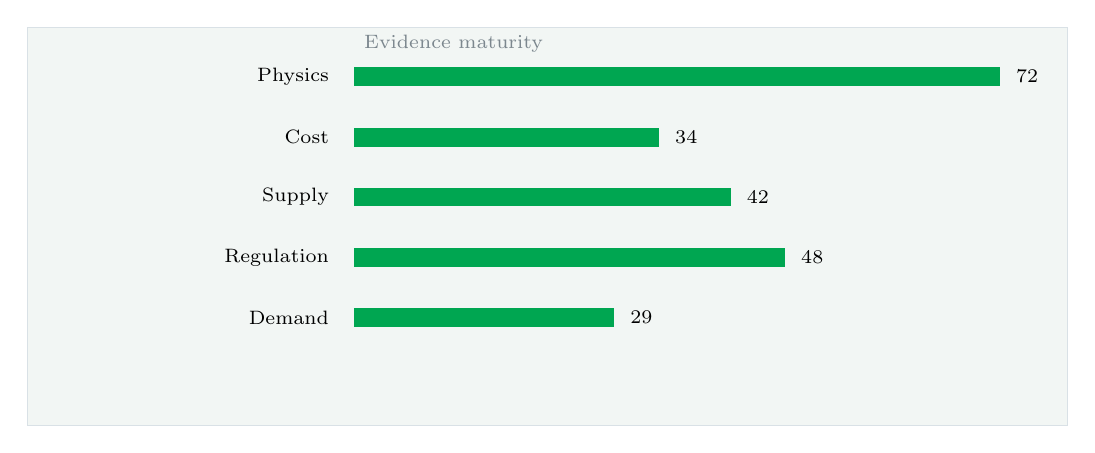
\begin{tikzpicture}[x=1cm,y=1cm]
\path[use as bounding box] (0,0) rectangle (13.20,5.05);
\fill[BOLight] (0,0) rectangle (13.20,5.05);
\draw[BOLine,line width=.35pt] (0,0) rectangle (13.20,5.05);
\node[anchor=west] at (4.15,4.85) {\scriptsize\color{BOMuted} Evidence maturity};
\node[anchor=east,align=right,text width=3.93cm] at (3.95,4.43) {\scriptsize Physics};
\fill[BOLight] (4.15,4.31) rectangle (12.35,4.55);
\fill[BOGreen] (4.15,4.31) rectangle (12.35,4.55);
\node[anchor=west] at (12.43,4.43) {\scriptsize 72};
\node[anchor=east,align=right,text width=3.93cm] at (3.95,3.66) {\scriptsize Cost};
\fill[BOLight] (4.15,3.54) rectangle (12.35,3.78);
\fill[BOGreen] (4.15,3.54) rectangle (8.02,3.78);
\node[anchor=west] at (8.10,3.66) {\scriptsize 34};
\node[anchor=east,align=right,text width=3.93cm] at (3.95,2.90) {\scriptsize Supply};
\fill[BOLight] (4.15,2.78) rectangle (12.35,3.02);
\fill[BOGreen] (4.15,2.78) rectangle (8.93,3.02);
\node[anchor=west] at (9.01,2.90) {\scriptsize 42};
\node[anchor=east,align=right,text width=3.93cm] at (3.95,2.13) {\scriptsize Regulation};
\fill[BOLight] (4.15,2.01) rectangle (12.35,2.25);
\fill[BOGreen] (4.15,2.01) rectangle (9.62,2.25);
\node[anchor=west] at (9.70,2.13) {\scriptsize 48};
\node[anchor=east,align=right,text width=3.93cm] at (3.95,1.37) {\scriptsize Demand};
\fill[BOLight] (4.15,1.25) rectangle (12.35,1.49);
\fill[BOGreen] (4.15,1.25) rectangle (7.45,1.49);
\node[anchor=west] at (7.53,1.37) {\scriptsize 29};
\end{tikzpicture}\par\vspace{2pt}
\vspace{1pt}\noindent\begin{minipage}[t]{0.56\linewidth}
{\footnotesize\color{BOText} Management can use the maturity gap to decide which claims support action today and which require a separate diligence workstream.}\par
\end{minipage}\hfill\begin{minipage}[t]{0.36\linewidth}
{\scriptsize\color{BOText}\begin{tabular}{p{31mm}>{\raggedleft\arraybackslash}p{18mm}}
\multicolumn{2}{l}{\textcolor{BOGreen}{\bfseries Visible readout}}\\[2pt]
Physics & \textbf{72}\\[1pt]
Cost & \textbf{34}\\[1pt]
Supply & \textbf{42}\\[1pt]
Regulation & \textbf{48}\\[1pt]
Demand & \textbf{29}\\[1pt]
\end{tabular}}\par
\end{minipage}\par\vspace{1pt}
\vspace{4pt}{\footnotesize\color{BOText} Management can use the maturity gap to decide which claims support action today and which require a separate diligence workstream.}\par
{\scriptsize\color{BOMuted} BlueOcean public-source synthesis.}\par

\clearpage
\label{chap:5}
\noindent\begin{tikzpicture}
\path[use as bounding box] (0,0) rectangle (\linewidth,54mm);
\clip (0,0) rectangle (\linewidth,54mm);
\node[anchor=north west,inner sep=0] at (0,54mm) {
\includegraphics[width=\linewidth]{assets/image-5.png}};
\end{tikzpicture}
\vspace{0pt}
\noindent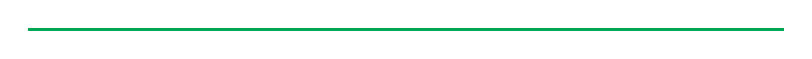
\begin{tikzpicture}
\fill[BOGreen] (0,0) rectangle (96mm,1.2pt);
\end{tikzpicture}\par\vspace{8pt}
{\Large\sffamily\bfseries\color{BONavy} Fusion\BOApos{}s Strategic Value Lies in Baseload Clean Power and Energy Independence, Not Near-Term Disruption}\par\vspace{4pt}
{\sffamily\fontsize{15}{20}\selectfont\color{BOGreen} Fusion is a long-term strategic asset for baseload clean power and energy security, not a near-term competitor to renewables. Position it as a hedge in energy portfolios.}\par\vspace{9pt}
\begin{multicols}{2}
{\small Fusion\BOApos{}s primary strategic value is as a source of baseload clean power. Unlike solar and wind, which are intermittent, fusion can provide continuous power, making it a complement to renewables in a decarbonized grid. Fusion also has a small land footprint and can be sited near population centers, reducing transmission costs.}\par
{\small Fusion could also enhance energy independence by reducing reliance on fossil fuel imports. Countries with abundant fusion fuel (deuterium from water, tritium bred from lithium) could achieve energy self-sufficiency. This has geopolitical implications, as it could shift the balance of energy power away from fossil fuel-rich nations.}\par
{\small However, fusion will not disrupt energy markets in the near term. Even under optimistic scenarios, commercial fusion is unlikely before 2040. By then, renewables and storage may have become even cheaper and more widespread. Fusion\BOApos{}s role will be to fill the gaps that renewables cannot easily address, such as providing reliable power during extended periods of low wind and solar output.}\par
{\small The cost of fusion must be competitive with other clean energy sources. Current projections for fusion LCOE range from \$50 to \$100 per MWh, but these are highly uncertain. If renewables plus storage can achieve LCOE below \$30/MWh by 2040, fusion may struggle to compete on cost alone. However, fusion may have value beyond electricity, such as providing high-temperature heat for industrial processes, which could command a premium.}\par
{\small For energy companies, fusion represents a long-term hedge. Investing now in fusion R\&D and partnerships builds knowledge and optionality. Companies that wait until fusion is proven may find themselves at a competitive disadvantage, as early movers will have established supply chains, regulatory relationships, and intellectual property.}\par
{\small The strategic implications for national security are also significant. Fusion could reduce dependence on foreign energy sources and provide a resilient power supply. Governments are likely to support fusion development for these reasons, creating a favorable policy environment.}\par
{\small In summary, fusion is not a near-term solution, but it is a critical long-term option. Companies and governments should invest now to secure a position in the fusion value chain, while managing risks through diversification and milestone-based approaches.}\par
{\small Management should identify which capabilities are scarce and can be secured early: critical supply, engineering delivery, channel partners, service network, financing partners and compliance capacity. Low-cost learning rights can be more valuable than waiting for full market clarity.}\par
\end{multicols}
\vspace{5pt}\noindent\begin{tabularx}{\linewidth}{Y Y Y}
{\textcolor{BOGreen}{\bfseries 01}}\par{\scriptsize\color{BOText} Fusion provides baseload clean power, complementing renewables} & {\textcolor{BOGreen}{\bfseries 02}}\par{\scriptsize\color{BOText} Not a near-term disruptor; commercial deployment likely post-2040} & {\textcolor{BOGreen}{\bfseries 03}}\par{\scriptsize\color{BOText} Strategic value as a long-term hedge and for energy independence} \\
\end{tabularx}\par\vspace{2pt}
\label{chap:5:end}

\clearpage
\label{chap:6}
\noindent\begin{tikzpicture}
\path[use as bounding box] (0,0) rectangle (\linewidth,54mm);
\clip (0,0) rectangle (\linewidth,54mm);
\node[anchor=north west,inner sep=0] at (0,54mm) {
\includegraphics[width=\linewidth]{assets/image-6.png}};
\end{tikzpicture}
\vspace{0pt}
\noindent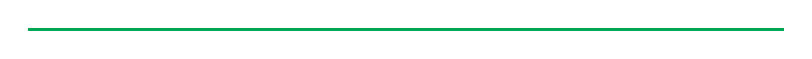
\begin{tikzpicture}
\fill[BOGreen] (0,0) rectangle (96mm,1.2pt);
\end{tikzpicture}\par\vspace{8pt}
{\Large\sffamily\bfseries\color{BONavy} Falling Costs of Renewables and Storage May Erode Fusion\BOApos{}s Competitive Advantage}\par\vspace{4pt}
{\sffamily\fontsize{15}{20}\selectfont\color{BOGreen} The rapid decline in renewable energy costs poses a challenge to fusion\BOApos{}s economic viability. Fusion cost targets must be benchmarked against realistic future energy prices.}\par\vspace{9pt}
\begin{multicols}{2}
{\small The cost of solar and wind energy has fallen dramatically over the past decade. Solar photovoltaic LCOE has declined by about 90\% since 2010, and onshore wind by about 70\%. Battery storage costs have also fallen sharply, by about 85\% since 2010. These trends are expected to continue, driven by manufacturing scale, technological improvements, and learning curves.}\par
{\small By 2030, solar LCOE is projected to be around \$20-30 per MWh in many regions, and solar-plus-storage could be \$30-50 per MWh. By 2040, these costs could be even lower. In contrast, fusion LCOE projections are highly uncertain, with estimates ranging from \$50 to \$100 per MWh. If fusion cannot achieve costs at the lower end of this range, it may struggle to compete with renewables on a pure cost basis.}\par
{\small However, fusion has advantages that renewables do not. It provides firm, dispatchable power, which is valuable for grid reliability. As the share of renewables increases, the value of firm power grows. In a high-renewables grid, the cost of balancing intermittent generation can be significant, and fusion could provide a cost-effective solution.}\par
{\small Fusion also has a much smaller land footprint than solar or wind farms, and it can be sited closer to demand centers, reducing transmission costs. These factors could make fusion economically attractive even if its LCOE is higher than that of renewables in some locations.}\par
{\small To remain competitive, fusion developers must focus on reducing capital costs and improving availability. The use of advanced manufacturing techniques, such as 3D printing and modular construction, could help. Additionally, fusion plants could be designed for cogeneration, producing hydrogen or heat for industrial use, which could improve economics.}\par
{\small Investors should benchmark fusion cost targets against realistic future energy prices, not current prices. A fusion plant that comes online in 2040 will compete against renewables and storage that have had another 15 years of cost declines. Sensitivity analysis should consider a range of renewable cost scenarios.}\par
{\small Policy support could also play a role. If governments value the reliability and energy security benefits of fusion, they may provide subsidies or guaranteed power purchase agreements, similar to those offered to nuclear and renewable projects. This could improve fusion\BOApos{}s economic viability.}\par
{\small No-regret moves include a sourced fact base, customer interviews, policy monitoring, supply-chain scans and small partner discussions. Option moves include pilots, preferential access and minority investments. Major commitments should wait for stronger proof.}\par
\end{multicols}
\vspace{5pt}\noindent\begin{tabularx}{\linewidth}{Y Y Y}
{\textcolor{BOGreen}{\bfseries 01}}\par{\scriptsize\color{BOText} Renewable costs have fallen dramatically and will continue to decline} & {\textcolor{BOGreen}{\bfseries 02}}\par{\scriptsize\color{BOText} Fusion must achieve LCOE at the lower end of projections to compete} & {\textcolor{BOGreen}{\bfseries 03}}\par{\scriptsize\color{BOText} Fusion\BOApos{}s firm power and small footprint provide value beyond LCOE} \\
\end{tabularx}\par\vspace{2pt}
\label{chap:6:end}

\clearpage
{\textcolor{BOGreen}{\scriptsize\bfseries EXHIBIT 11}}\par\vspace{4pt}
{\sffamily\fontsize{17}{21}\selectfont\color{BONavy} Use-case priorities separate early revenue from long-term optionality}\par
{\small\color{BOText} Customer option screen for Nuclear Fusion Commercialization Outlook and Strategic Implications}\par\vspace{6pt}
\noindent\fcolorbox{BOLine}{BOLight}{\begin{minipage}{0.96\linewidth}\vspace{4pt}{\scriptsize\begin{tabular}{p{38mm}>{\centering\arraybackslash}p{21mm}>{\centering\arraybackslash}p{21mm}>{\centering\arraybackslash}p{21mm}>{\centering\arraybackslash}p{21mm}}
 & {\bfseries Demand pull} & {\bfseries Price tolerance} & {\bfseries Timing} & {\bfseries Evidence} \\
\hline
{\bfseries Industrial heat} & \colorbox{BOGreen}{\textcolor{white}{\strut\hspace{5pt}5\hspace{5pt}}} & \colorbox{BOGreen}{\textcolor{white}{\strut\hspace{5pt}4\hspace{5pt}}} & \colorbox{BOBlue}{\textcolor{white}{\strut\hspace{5pt}3\hspace{5pt}}} & \colorbox{BOBlue}{\textcolor{white}{\strut\hspace{5pt}3\hspace{5pt}}} \\
{\bfseries Hydrogen} & \colorbox{BOGreen}{\textcolor{white}{\strut\hspace{5pt}4\hspace{5pt}}} & \colorbox{BOGreen}{\textcolor{white}{\strut\hspace{5pt}4\hspace{5pt}}} & \colorbox{BOBlue}{\textcolor{white}{\strut\hspace{5pt}3\hspace{5pt}}} & \colorbox{BOLight}{\textcolor{BOText}{\strut\hspace{5pt}2\hspace{5pt}}} \\
{\bfseries Grid power} & \colorbox{BOGreen}{\textcolor{white}{\strut\hspace{5pt}5\hspace{5pt}}} & \colorbox{BOLight}{\textcolor{BOText}{\strut\hspace{5pt}2\hspace{5pt}}} & \colorbox{BOLight}{\textcolor{BOText}{\strut\hspace{5pt}1\hspace{5pt}}} & \colorbox{BOLight}{\textcolor{BOText}{\strut\hspace{5pt}2\hspace{5pt}}} \\
{\bfseries Defense / remote} & \colorbox{BOBlue}{\textcolor{white}{\strut\hspace{5pt}3\hspace{5pt}}} & \colorbox{BOGreen}{\textcolor{white}{\strut\hspace{5pt}5\hspace{5pt}}} & \colorbox{BOBlue}{\textcolor{white}{\strut\hspace{5pt}3\hspace{5pt}}} & \colorbox{BOLight}{\textcolor{BOText}{\strut\hspace{5pt}2\hspace{5pt}}} \\
{\bfseries Research services} & \colorbox{BOLight}{\textcolor{BOText}{\strut\hspace{5pt}2\hspace{5pt}}} & \colorbox{BOBlue}{\textcolor{white}{\strut\hspace{5pt}3\hspace{5pt}}} & \colorbox{BOGreen}{\textcolor{white}{\strut\hspace{5pt}4\hspace{5pt}}} & \colorbox{BOGreen}{\textcolor{white}{\strut\hspace{5pt}4\hspace{5pt}}} \\
\end{tabular}}\vspace{4pt}\end{minipage}}\par\vspace{2pt}
\vspace{1pt}\noindent\begin{minipage}[t]{0.56\linewidth}
{\footnotesize\color{BOText} The comparison separates markets that can teach the company soon from markets that may require longer proof cycles.}\par
\end{minipage}\hfill\begin{minipage}[t]{0.36\linewidth}
{\scriptsize\color{BOText}\begin{tabular}{p{31mm}>{\raggedleft\arraybackslash}p{18mm}}
\multicolumn{2}{l}{\textcolor{BOGreen}{\bfseries Matrix readout}}\\[2pt]
Industrial heat & \textbf{5 / 4}\\[1pt]
Hydrogen & \textbf{4 / 4}\\[1pt]
Grid power & \textbf{5 / 2}\\[1pt]
Defense / remote & \textbf{3 / 5}\\[1pt]
\end{tabular}}\par
\end{minipage}\par\vspace{1pt}
\vspace{4pt}{\footnotesize\color{BOText} The comparison separates markets that can teach the company soon from markets that may require longer proof cycles.}\par
{\scriptsize\color{BOMuted} BlueOcean customer option synthesis.}\par
\vspace{9pt}\textcolor{BOLine}{\rule{\linewidth}{0.3pt}}\vspace{8pt}
{\textcolor{BOGreen}{\scriptsize\bfseries EXHIBIT 12}}\par\vspace{4pt}
{\sffamily\fontsize{17}{21}\selectfont\color{BONavy} Capital exposure should be staged by decision milestone}\par
{\small\color{BOText} Commitment profile for Nuclear Fusion Commercialization Outlook and Strategic Implications}\par\vspace{6pt}
\noindent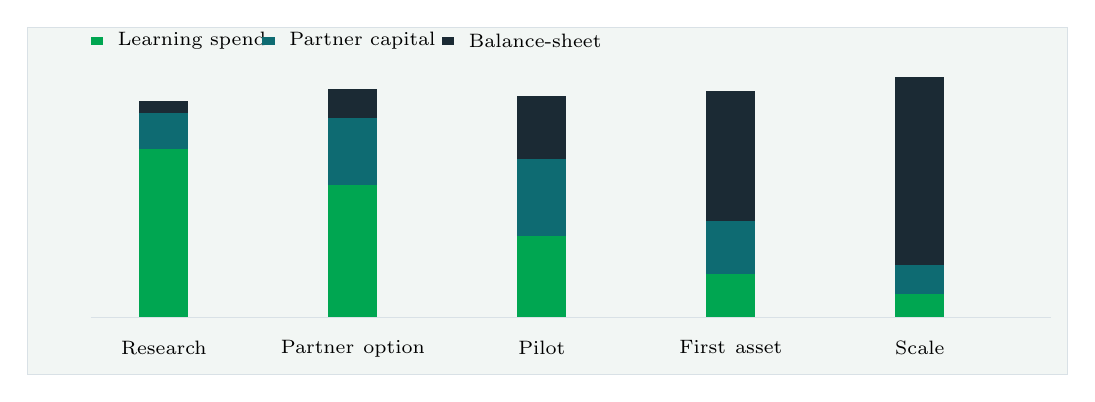
\begin{tikzpicture}[x=1cm,y=1cm]
\path[use as bounding box] (0,0) rectangle (13.20,4.40);
\fill[BOLight] (0,0) rectangle (13.20,4.40);
\draw[BOLine,line width=.35pt] (0,0) rectangle (13.20,4.40);
\draw[BOLine] (0.80,0.72) -- (13.00,0.72);
\fill[BOGreen] (1.42,0.72) rectangle (2.04,2.86);
\fill[BOBlue] (1.42,2.86) rectangle (2.04,3.31);
\fill[BONavy] (1.42,3.31) rectangle (2.04,3.47);
\node[anchor=north,align=center,text width=2.21cm] at (1.73,0.55) {\scriptsize Research};
\fill[BOGreen] (3.82,0.72) rectangle (4.44,2.40);
\fill[BOBlue] (3.82,2.40) rectangle (4.44,3.25);
\fill[BONavy] (3.82,3.25) rectangle (4.44,3.62);
\node[anchor=north,align=center,text width=2.21cm] at (4.13,0.55) {\scriptsize Partner option};
\fill[BOGreen] (6.22,0.72) rectangle (6.84,1.76);
\fill[BOBlue] (6.22,1.76) rectangle (6.84,2.73);
\fill[BONavy] (6.22,2.73) rectangle (6.84,3.53);
\node[anchor=north,align=center,text width=2.21cm] at (6.53,0.55) {\scriptsize Pilot};
\fill[BOGreen] (8.62,0.72) rectangle (9.24,1.27);
\fill[BOBlue] (8.62,1.27) rectangle (9.24,1.94);
\fill[BONavy] (8.62,1.94) rectangle (9.24,3.59);
\node[anchor=north,align=center,text width=2.21cm] at (8.93,0.55) {\scriptsize First asset};
\fill[BOGreen] (11.02,0.72) rectangle (11.64,1.02);
\fill[BOBlue] (11.02,1.02) rectangle (11.64,1.39);
\fill[BONavy] (11.02,1.39) rectangle (11.64,3.77);
\node[anchor=north,align=center,text width=2.21cm] at (11.33,0.55) {\scriptsize Scale};
\fill[BOGreen] (0.80,4.18) rectangle (0.96,4.28);
\node[anchor=west] at (1.02,4.23) {\scriptsize Learning spend};
\fill[BOBlue] (2.98,4.18) rectangle (3.14,4.28);
\node[anchor=west] at (3.20,4.23) {\scriptsize Partner capital};
\fill[BONavy] (5.26,4.18) rectangle (5.42,4.28);
\node[anchor=west] at (5.48,4.23) {\scriptsize Balance-sheet};
\end{tikzpicture}\par\vspace{2pt}
\vspace{1pt}\noindent\begin{minipage}[t]{0.56\linewidth}
{\footnotesize\color{BOText} The capital mix should move from learning to committed exposure only as evidence matures.}\par
\end{minipage}\hfill\begin{minipage}[t]{0.36\linewidth}
{\scriptsize\color{BOText}\begin{tabular}{p{31mm}>{\raggedleft\arraybackslash}p{18mm}}
\multicolumn{2}{l}{\textcolor{BOGreen}{\bfseries Visible readout}}\\[2pt]
Research & \textbf{90}\\[1pt]
Partner option & \textbf{95}\\[1pt]
Pilot & \textbf{92}\\[1pt]
First asset & \textbf{94}\\[1pt]
Scale & \textbf{100}\\[1pt]
\end{tabular}}\par
\end{minipage}\par\vspace{1pt}
\vspace{4pt}{\footnotesize\color{BOText} The capital mix should move from learning to committed exposure only as evidence matures.}\par
{\scriptsize\color{BOMuted} BlueOcean capital staging view.}\par

\clearpage
\label{chap:7}
\noindent\begin{tikzpicture}
\path[use as bounding box] (0,0) rectangle (\linewidth,54mm);
\clip (0,0) rectangle (\linewidth,54mm);
\node[anchor=north west,inner sep=0] at (0,54mm) {
\includegraphics[width=\linewidth]{assets/image-7.png}};
\end{tikzpicture}
\vspace{0pt}
\noindent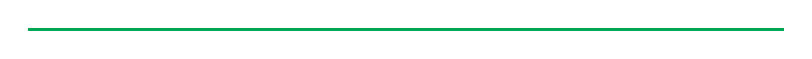
\begin{tikzpicture}
\fill[BOGreen] (0,0) rectangle (96mm,1.2pt);
\end{tikzpicture}\par\vspace{8pt}
{\Large\sffamily\bfseries\color{BONavy} Geopolitical Dynamics Are Shaping Fusion R\&D Leadership}\par\vspace{4pt}
{\sffamily\fontsize{15}{20}\selectfont\color{BOGreen} The U.S., China, and Europe are the key players in fusion R\&D. Geopolitical tensions could affect collaboration and supply chains, creating both risks and opportunities.}\par\vspace{9pt}
\begin{multicols}{2}
{\small Fusion research and development is a global endeavor, but the leadership landscape is shifting. The United States has long been a leader in fusion science, with major facilities like the National Ignition Facility (NIF) and the DIII-D tokamak. In recent years, the U.S. has also become a hub for private fusion investment, with companies like CFS, TAE, and Helion based in the country.}\par
{\small China is rapidly advancing its fusion program. The EAST tokamak has achieved long-pulse plasma operation, and China is a key partner in ITER. China is also building its own fusion reactor, the China Fusion Engineering Test Reactor (CFETR), which aims to demonstrate tritium breeding and steady-state operation. China\BOApos{}s state-backed approach allows for large-scale, long-term investment.}\par
{\small Europe, through the ITER project and national programs, remains a major player. The UK has its own fusion strategy, including the STEP (Spherical Tokamak for Energy Production) program, which aims to build a prototype fusion plant by 2040. Germany\BOApos{}s Wendelstein 7-X stellarator is a world-class facility.}\par
{\small Geopolitical tensions, particularly between the U.S. and China, could affect fusion collaboration. Export controls on sensitive technologies, such as high-temperature superconductors and tritium handling equipment, could fragment global supply chains. Companies may need to develop domestic alternatives or diversify suppliers.}\par
{\small On the other hand, fusion could be an area for international cooperation, as it is a global public good. The ITER project is a model of multinational collaboration, though it has faced challenges. New initiatives, such as the IAEA\BOApos{}s fusion roadmap, aim to foster collaboration.}\par
{\small For companies, the geopolitical landscape creates both risks and opportunities. Investing in multiple regions can mitigate risk, but it also requires navigating different regulatory and political environments. Partnerships with companies in allied countries may be more stable than those with potential adversaries.}\par
{\small The race for fusion leadership could also have implications for intellectual property. Companies that develop key technologies may gain a competitive advantage, but they may also face pressure to share technology for the greater good. Patent strategies and licensing agreements will be important.}\par
{\small Near-term work should close source, customer, cost and timeline gaps; medium-term work should test pilots and partners; long-term work should cover capital, M\&A or scaled entry only when proof is strong enough.}\par
\end{multicols}
\vspace{5pt}\noindent\begin{tabularx}{\linewidth}{Y Y Y}
{\textcolor{BOGreen}{\bfseries 01}}\par{\scriptsize\color{BOText} U.S., China, and Europe are key players in fusion R\&D} & {\textcolor{BOGreen}{\bfseries 02}}\par{\scriptsize\color{BOText} Geopolitical tensions could affect collaboration and supply chains} & {\textcolor{BOGreen}{\bfseries 03}}\par{\scriptsize\color{BOText} Diversify geographic exposure and build partnerships in allied countries} \\
\end{tabularx}\par\vspace{2pt}
\label{chap:7:end}

\clearpage
\label{chap:8}
\noindent\begin{tikzpicture}
\path[use as bounding box] (0,0) rectangle (\linewidth,54mm);
\clip (0,0) rectangle (\linewidth,54mm);
\node[anchor=north west,inner sep=0] at (0,54mm) {
\includegraphics[width=\linewidth]{assets/image-8.png}};
\end{tikzpicture}
\vspace{0pt}
\noindent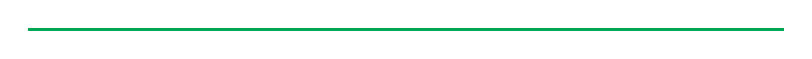
\begin{tikzpicture}
\fill[BOGreen] (0,0) rectangle (96mm,1.2pt);
\end{tikzpicture}\par\vspace{8pt}
{\Large\sffamily\bfseries\color{BONavy} Recommendations for Decision-Makers}\par\vspace{4pt}
{\sffamily\fontsize{15}{20}\selectfont\color{BOGreen} Based on the analysis, we recommend a phased approach to fusion investment, focusing on diversification, milestone-based commitments, and early regulatory engagement.}\par\vspace{9pt}
\begin{multicols}{2}
{\small For corporate leaders, the key is to build a strategic position in fusion without over-committing. The technology is promising but unproven, and the timeline is long. A phased approach allows for learning and adjustment as the technology matures.}\par
{\small A practical reading is that for investors, the key is to focus on technical milestones, not just funding amounts. Look for companies with credible physics, experienced teams, and clear development plans. A portfolio approach across multiple designs and stages reduces risk.}\par
{\small For policymakers, the key is to accelerate regulatory development and provide support for fusion R\&D. The U.S. DOE\BOApos{}s Milestone-Based Fusion Development Program is a good model. International collaboration should be encouraged, but with safeguards for sensitive technologies.}\par
{\small For capital allocation, management should not treat media attention, financing announcements or single technical claims as decision signals on their own. More useful signals include customer procurement, cost movement, regulatory clarity, competitor commitments and financing terms.}\par
{\small In conclusion, fusion is a long-term strategic opportunity that requires patient capital and careful risk management. By taking a phased, diversified approach, decision-makers can position themselves to benefit from fusion\BOApos{}s potential while avoiding the pitfalls of over-commitment.}\par
{\small In the long term (5-10 years), prepare for fusion integration into energy portfolios. Develop offtake agreements with fusion developers and plan for grid interconnection. Monitor technology milestones and adjust investment strategy accordingly.}\par
{\small In the medium term (2-5 years), engage with regulators and industry consortia to shape fusion licensing frameworks. Participate in regulatory working groups and develop internal expertise on fusion regulation. This positions the company to be a first-mover when regulatory clarity emerges.}\par
{\small In the near term (0-2 years), establish a fusion scouting and investment team. Conduct due diligence on leading private ventures and enabling technologies. Make initial investments in a diversified portfolio of 2-3 companies, with milestone-based tranches. This provides upside exposure while limiting downside risk.}\par
\end{multicols}
\vspace{5pt}\noindent\begin{tabularx}{\linewidth}{Y Y Y}
{\textcolor{BOGreen}{\bfseries 01}}\par{\scriptsize\color{BOText} Phased approach: scout, invest, engage, prepare} & {\textcolor{BOGreen}{\bfseries 02}}\par{\scriptsize\color{BOText} Diversify across fusion approaches and enabling technologies} & {\textcolor{BOGreen}{\bfseries 03}}\par{\scriptsize\color{BOText} Use milestone-based tranches to manage risk} \\
\end{tabularx}\par\vspace{2pt}
\label{chap:8:end}

\clearpage
{\textcolor{BOGreen}{\scriptsize\bfseries EXHIBIT 13}}\par\vspace{4pt}
{\sffamily\fontsize{17}{21}\selectfont\color{BONavy} Management attention shifts as the uncertainty stack resolves}\par
{\small\color{BOText} Executive review cadence for Nuclear Fusion Commercialization Outlook and Strategic Implications}\par\vspace{6pt}
\noindent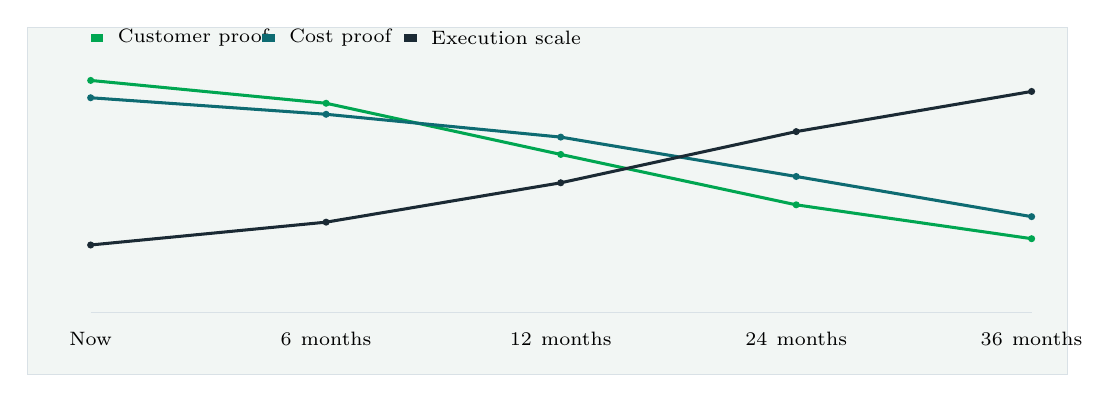
\begin{tikzpicture}[x=1cm,y=1cm]
\path[use as bounding box] (0,0) rectangle (13.20,4.40);
\fill[BOLight] (0,0) rectangle (13.20,4.40);
\draw[BOLine,line width=.35pt] (0,0) rectangle (13.20,4.40);
\draw[BOLine] (0.80,0.78) -- (12.75,0.78);
\draw[BOGreen,line width=1.1pt] (0.80,3.73) -- (3.79,3.44) -- (6.77,2.79) -- (9.76,2.15) -- (12.75,1.72);
\fill[BOGreen] (0.80,3.73) circle (.045);
\fill[BOGreen] (3.79,3.44) circle (.045);
\fill[BOGreen] (6.77,2.79) circle (.045);
\fill[BOGreen] (9.76,2.15) circle (.045);
\fill[BOGreen] (12.75,1.72) circle (.045);
\draw[BOBlue,line width=1.1pt] (0.80,3.51) -- (3.79,3.30) -- (6.77,3.01) -- (9.76,2.51) -- (12.75,2.00);
\fill[BOBlue] (0.80,3.51) circle (.045);
\fill[BOBlue] (3.79,3.30) circle (.045);
\fill[BOBlue] (6.77,3.01) circle (.045);
\fill[BOBlue] (9.76,2.51) circle (.045);
\fill[BOBlue] (12.75,2.00) circle (.045);
\draw[BONavy,line width=1.1pt] (0.80,1.64) -- (3.79,1.93) -- (6.77,2.43) -- (9.76,3.08) -- (12.75,3.59);
\fill[BONavy] (0.80,1.64) circle (.045);
\fill[BONavy] (3.79,1.93) circle (.045);
\fill[BONavy] (6.77,2.43) circle (.045);
\fill[BONavy] (9.76,3.08) circle (.045);
\fill[BONavy] (12.75,3.59) circle (.045);
\node[anchor=north,align=center,text width=1.8cm] at (0.80,0.66) {\scriptsize Now};
\node[anchor=north,align=center,text width=1.8cm] at (3.79,0.66) {\scriptsize 6 months};
\node[anchor=north,align=center,text width=1.8cm] at (6.77,0.66) {\scriptsize 12 months};
\node[anchor=north,align=center,text width=1.8cm] at (9.76,0.66) {\scriptsize 24 months};
\node[anchor=north,align=center,text width=1.8cm] at (12.75,0.66) {\scriptsize 36 months};
\fill[BOGreen] (0.80,4.22) rectangle (0.96,4.32);
\node[anchor=west] at (1.02,4.27) {\scriptsize Customer proof};
\fill[BOBlue] (2.98,4.22) rectangle (3.14,4.32);
\node[anchor=west] at (3.20,4.27) {\scriptsize Cost proof};
\fill[BONavy] (4.78,4.22) rectangle (4.94,4.32);
\node[anchor=west] at (5.00,4.27) {\scriptsize Execution scale};
\end{tikzpicture}\par\vspace{2pt}
\vspace{1pt}\noindent\begin{minipage}[t]{0.56\linewidth}
{\footnotesize\color{BOText} The review agenda should shift from proof gathering toward scaling questions only after the earlier uncertainties narrow.}\par
\end{minipage}\hfill\begin{minipage}[t]{0.36\linewidth}
{\scriptsize\color{BOText}\begin{tabular}{p{31mm}>{\raggedleft\arraybackslash}p{18mm}}
\multicolumn{2}{l}{\textcolor{BOGreen}{\bfseries Visible readout}}\\[2pt]
Now & \textbf{182}\\[1pt]
6 months & \textbf{176}\\[1pt]
12 months & \textbf{164}\\[1pt]
24 months & \textbf{150}\\[1pt]
36 months & \textbf{138}\\[1pt]
\end{tabular}}\par
\end{minipage}\par\vspace{1pt}
\vspace{4pt}{\footnotesize\color{BOText} The review agenda should shift from proof gathering toward scaling questions only after the earlier uncertainties narrow.}\par
{\scriptsize\color{BOMuted} BlueOcean uncertainty-resolution model.}\par
\vspace{9pt}\textcolor{BOLine}{\rule{\linewidth}{0.3pt}}\vspace{8pt}
{\textcolor{BOGreen}{\scriptsize\bfseries EXHIBIT 14}}\par\vspace{4pt}
{\sffamily\fontsize{17}{21}\selectfont\color{BONavy} Competitive posture depends on timing, access and reversibility}\par
{\small\color{BOText} Strategic posture map for Nuclear Fusion Commercialization Outlook and Strategic Implications}\par\vspace{6pt}
\noindent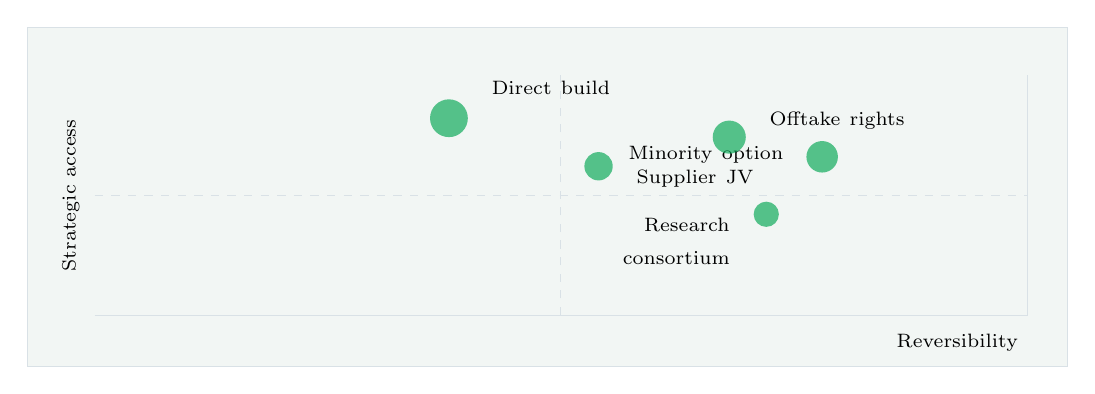
\begin{tikzpicture}[x=1cm,y=1cm]
\path[use as bounding box] (0,0) rectangle (13.20,4.30);
\fill[BOLight] (0,0) rectangle (13.20,4.30);
\draw[BOLine,line width=.35pt] (0,0) rectangle (13.20,4.30);
\draw[BOLine] (0.85,0.65) -- (12.70,0.65) -- (12.70,3.70);
\draw[BOLine,dashed] (0.85,2.17) -- (12.70,2.17);
\draw[BOLine,dashed] (6.77,0.65) -- (6.77,3.70);
\fill[BOGreen,opacity=.65] (10.09,2.66) circle (0.20);
\node[anchor=east,align=right,text width=2.10cm] at (9.72,2.69) {\scriptsize Minority option};
\fill[BOGreen,opacity=.65] (8.91,2.91) circle (0.21);
\node[anchor=west,align=left,text width=2.10cm] at (9.30,3.12) {\scriptsize Offtake rights};
\fill[BOGreen,opacity=.65] (7.25,2.54) circle (0.18);
\node[anchor=west,align=left,text width=2.10cm] at (7.61,2.38) {\scriptsize Supplier JV};
\fill[BOGreen,opacity=.65] (5.35,3.15) circle (0.24);
\node[anchor=west,align=left,text width=2.10cm] at (5.77,3.54) {\scriptsize Direct build};
\fill[BOGreen,opacity=.65] (9.38,1.93) circle (0.16);
\node[anchor=east,align=right,text width=2.10cm] at (9.04,1.59) {\scriptsize Research consortium};
\node[anchor=north east] at (12.70,0.53) {\scriptsize Reversibility};
\node[anchor=center,rotate=90] at (0.55,2.17) {\scriptsize Strategic access};
\end{tikzpicture}\par\vspace{2pt}
\vspace{1pt}\noindent\begin{minipage}[t]{0.56\linewidth}
{\footnotesize\color{BOText} Early moves should protect access and learning while avoiding positions that cannot be reversed if evidence weakens.}\par
\end{minipage}\hfill\begin{minipage}[t]{0.36\linewidth}
{\scriptsize\color{BOText}\begin{tabular}{p{31mm}>{\raggedleft\arraybackslash}p{18mm}}
\multicolumn{2}{l}{\textcolor{BOGreen}{\bfseries Position}}\\[2pt]
Minority option & \textbf{78 / 66}\\[1pt]
Offtake rights & \textbf{68 / 74}\\[1pt]
Supplier JV & \textbf{54 / 62}\\[1pt]
Direct build & \textbf{38 / 82}\\[1pt]
Research consortium & \textbf{72 / 42}\\[1pt]
\end{tabular}}\par
\end{minipage}\par\vspace{1pt}
\vspace{4pt}{\footnotesize\color{BOText} Early moves should protect access and learning while avoiding positions that cannot be reversed if evidence weakens.}\par
{\scriptsize\color{BOMuted} BlueOcean competitive posture screen.}\par

\clearpage
{\sffamily\fontsize{20}{25}\selectfont\color{BONavy} About the research}\par\vspace{6pt}
\vspace{2pt}{\color{BOBright}\rule{\linewidth}{1pt}}\vspace{5pt}
{\footnotesize\color{BOMuted} This report has been prepared for strategy discussion and executive decision support. It is not investment, legal, tax, audit or valuation advice. Market estimates, forecasts and scenarios are directional and should be independently validated before they are used for investment, financing, transaction, regulatory or operational decisions. Forward-looking views may change as technology, policy, financing, regulation, competition, supply chains and macro conditions evolve. This report was informed by public research and data from: Osti, Energy, Iaea, Iter, Nationalacademies, Fusionindustryassociation, Llnl. Detailed references are retained separately rather than reproduced in the client-facing document. Recipients should perform their own diligence and treat this report as one input into a broader decision process.}

\clearpage
\noindent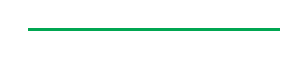
\begin{tikzpicture}
\fill[BOGreen] (0,0) rectangle (32mm,1.2pt);
\end{tikzpicture}\par\vspace{8pt}
{\sffamily\fontsize{24}{30}\selectfont\color{BONavy} About BlueOcean}\par\vspace{10pt}
\begin{minipage}[t]{0.44\linewidth}
{\sffamily\fontsize{16}{22}\selectfont\color{BOGreen} Research is most useful when it changes a management decision.}\par\vspace{8pt}
{\footnotesize\color{BOText} BlueOcean prepares decision-focused research for executives who need to separate credible evidence from market noise, translate technology shifts into commercial implications and stage commitments around proof.}\par\vspace{7pt}
{\footnotesize\color{BOMuted} This report draws on Osti, Energy, Iaea, Iter, Nationalacademies, Fusionindustryassociation, Llnl.}\par
\end{minipage}\hfill\begin{minipage}[t]{0.48\linewidth}
\begin{tabularx}{\linewidth}{p{31mm}Y}
{\small\bfseries This report was prepared by a strategic research team with expertise in energy}\par{\scriptsize\color{BOGreen} Research synthesis team} & {\footnotesize Responsible for evidence checks, executive synthesis and report QA.} \\[7pt]
\end{tabularx}
\end{minipage}


\clearpage
\thispagestyle{empty}
\begin{tikzpicture}[remember picture,overlay]
\node[anchor=south west,inner sep=0] at (current page.south west) {
\includegraphics[width=\paperwidth,height=\paperheight]{assets/cover-ai.png}};
\fill[black,opacity=.45] (current page.south west) rectangle (current page.north east);
\node[anchor=south east] at ([xshift=-11mm,yshift=10mm]current page.south east) {\sffamily\bfseries\Large\color{white} BlueOcean};
\end{tikzpicture}

\end{document}
